\documentclass[11pt]{article}

% The four macros of the header standard; tools/zenodo/publish_revision.py patches them when it reserves the DOI.
\newcommand{\doctype}{Preprint}
\newcommand{\docversion}{v1.00.000}
\newcommand{\docdate}{4 November 2026}
\newcommand{\versiondoi}{10.5281/zenodo.0}
\newcommand{\conceptdoi}{10.5281/zenodo.0}
\newcommand{\docidentity}{CAOS\_Contraste, the validation of the risk models of a bank}

% The packages and conventions every Contraste manuscript shares (CAOS_MANAGE conventions/manuscript-content-bar.md
% section 2). A document sets its class, the four header macros and \docidentity, then % The packages and conventions every Contraste manuscript shares (CAOS_MANAGE conventions/manuscript-content-bar.md
% section 2). A document sets its class, the four header macros and \docidentity, then % The packages and conventions every Contraste manuscript shares (CAOS_MANAGE conventions/manuscript-content-bar.md
% section 2). A document sets its class, the four header macros and \docidentity, then \input{../_shared/preamble}.
\usepackage[T1]{fontenc}
\usepackage[utf8]{inputenc}
\usepackage{lmodern}
\usepackage{microtype}
\usepackage[a4paper,margin=2.5cm]{geometry}
\usepackage{amsmath,amssymb,amsthm,mathtools,bm}
\usepackage{graphicx}
\usepackage{booktabs,longtable,tabularx,array,multirow}
\usepackage{siunitx}
\usepackage{algorithm}
\usepackage{algpseudocode}
\usepackage{caption,subcaption}
\usepackage{xcolor}
\usepackage[numbers,sort&compress]{natbib}
\usepackage[hidelinks]{hyperref}
\usepackage{cleveref}
\usepackage{orcidlink}

\sisetup{group-separator={,},group-minimum-digits=4,detect-all}
\graphicspath{{figures/}{../figures/}}
\captionsetup{font=small,labelfont=bf}
\setlength{\LTcapwidth}{\textwidth}

% Theorem environments for the Theory sections of the manuscripts.
\newtheorem{proposition}{Proposition}
\newtheorem{lemma}{Lemma}
\newtheorem{corollary}{Corollary}
\theoremstyle{definition}
\newtheorem{definition}{Definition}
\newtheorem{assumption}{Assumption}
\theoremstyle{remark}
\newtheorem{remark}{Remark}

% Notation shared by the documents (each defines it again in its notation table).
\newcommand{\E}{\mathbb{E}}
\newcommand{\Prob}{\mathbb{P}}
\newcommand{\Var}{\operatorname{Var}}
\newcommand{\Cov}{\operatorname{Cov}}
\newcommand{\VaR}{\operatorname{VaR}}
\newcommand{\ES}{\operatorname{ES}}
\newcommand{\PD}{\mathrm{PD}}
\newcommand{\LGD}{\mathrm{LGD}}
\newcommand{\EAD}{\mathrm{EAD}}
\newcommand{\ECL}{\mathrm{ECL}}
\newcommand{\indic}{\mathbf{1}}
\newcommand{\R}{\mathbb{R}}
\newcommand{\dd}{\,\mathrm{d}}

% The page-1 header block (CAOS_MANAGE conventions/manuscript-header-standard.md). The document defines \doctype,
% \docversion, \docdate, \versiondoi, \conceptdoi and \docidentity before this file; the publishing tool patches the four
% macros of the standard when it reserves the version DOI.
\newcommand{\docrepo}{github.com/fsantibanezleal/CAOS\_Contraste}
\newcommand{\headerblock}{%
\begin{center}
\fbox{\parbox{0.94\textwidth}{\small\raggedright
\textbf{\doctype} \quad$\cdot$\quad \docversion, \docdate \quad$\cdot$\quad Licence CC BY 4.0\\[2pt]
CAOS open-research programme \quad$\cdot$\quad \docidentity\\[2pt]
Version DOI \href{https://doi.org/\versiondoi}{\texttt{\versiondoi}} \quad$\cdot$\quad
concept DOI (always latest) \href{https://doi.org/\conceptdoi}{\texttt{\conceptdoi}}\\[2pt]
Not peer reviewed. Source code, data and computational records: \href{https://\docrepo}{\texttt{\docrepo}}
}}
\end{center}
\vspace{4pt}}
.
\usepackage[T1]{fontenc}
\usepackage[utf8]{inputenc}
\usepackage{lmodern}
\usepackage{microtype}
\usepackage[a4paper,margin=2.5cm]{geometry}
\usepackage{amsmath,amssymb,amsthm,mathtools,bm}
\usepackage{graphicx}
\usepackage{booktabs,longtable,tabularx,array,multirow}
\usepackage{siunitx}
\usepackage{algorithm}
\usepackage{algpseudocode}
\usepackage{caption,subcaption}
\usepackage{xcolor}
\usepackage[numbers,sort&compress]{natbib}
\usepackage[hidelinks]{hyperref}
\usepackage{cleveref}
\usepackage{orcidlink}

\sisetup{group-separator={,},group-minimum-digits=4,detect-all}
\graphicspath{{figures/}{../figures/}}
\captionsetup{font=small,labelfont=bf}
\setlength{\LTcapwidth}{\textwidth}

% Theorem environments for the Theory sections of the manuscripts.
\newtheorem{proposition}{Proposition}
\newtheorem{lemma}{Lemma}
\newtheorem{corollary}{Corollary}
\theoremstyle{definition}
\newtheorem{definition}{Definition}
\newtheorem{assumption}{Assumption}
\theoremstyle{remark}
\newtheorem{remark}{Remark}

% Notation shared by the documents (each defines it again in its notation table).
\newcommand{\E}{\mathbb{E}}
\newcommand{\Prob}{\mathbb{P}}
\newcommand{\Var}{\operatorname{Var}}
\newcommand{\Cov}{\operatorname{Cov}}
\newcommand{\VaR}{\operatorname{VaR}}
\newcommand{\ES}{\operatorname{ES}}
\newcommand{\PD}{\mathrm{PD}}
\newcommand{\LGD}{\mathrm{LGD}}
\newcommand{\EAD}{\mathrm{EAD}}
\newcommand{\ECL}{\mathrm{ECL}}
\newcommand{\indic}{\mathbf{1}}
\newcommand{\R}{\mathbb{R}}
\newcommand{\dd}{\,\mathrm{d}}

% The page-1 header block (CAOS_MANAGE conventions/manuscript-header-standard.md). The document defines \doctype,
% \docversion, \docdate, \versiondoi, \conceptdoi and \docidentity before this file; the publishing tool patches the four
% macros of the standard when it reserves the version DOI.
\newcommand{\docrepo}{github.com/fsantibanezleal/CAOS\_Contraste}
\newcommand{\headerblock}{%
\begin{center}
\fbox{\parbox{0.94\textwidth}{\small\raggedright
\textbf{\doctype} \quad$\cdot$\quad \docversion, \docdate \quad$\cdot$\quad Licence CC BY 4.0\\[2pt]
CAOS open-research programme \quad$\cdot$\quad \docidentity\\[2pt]
Version DOI \href{https://doi.org/\versiondoi}{\texttt{\versiondoi}} \quad$\cdot$\quad
concept DOI (always latest) \href{https://doi.org/\conceptdoi}{\texttt{\conceptdoi}}\\[2pt]
Not peer reviewed. Source code, data and computational records: \href{https://\docrepo}{\texttt{\docrepo}}
}}
\end{center}
\vspace{4pt}}
.
\usepackage[T1]{fontenc}
\usepackage[utf8]{inputenc}
\usepackage{lmodern}
\usepackage{microtype}
\usepackage[a4paper,margin=2.5cm]{geometry}
\usepackage{amsmath,amssymb,amsthm,mathtools,bm}
\usepackage{graphicx}
\usepackage{booktabs,longtable,tabularx,array,multirow}
\usepackage{siunitx}
\usepackage{algorithm}
\usepackage{algpseudocode}
\usepackage{caption,subcaption}
\usepackage{xcolor}
\usepackage[numbers,sort&compress]{natbib}
\usepackage[hidelinks]{hyperref}
\usepackage{cleveref}
\usepackage{orcidlink}

\sisetup{group-separator={,},group-minimum-digits=4,detect-all}
\graphicspath{{figures/}{../figures/}}
\captionsetup{font=small,labelfont=bf}
\setlength{\LTcapwidth}{\textwidth}

% Theorem environments for the Theory sections of the manuscripts.
\newtheorem{proposition}{Proposition}
\newtheorem{lemma}{Lemma}
\newtheorem{corollary}{Corollary}
\theoremstyle{definition}
\newtheorem{definition}{Definition}
\newtheorem{assumption}{Assumption}
\theoremstyle{remark}
\newtheorem{remark}{Remark}

% Notation shared by the documents (each defines it again in its notation table).
\newcommand{\E}{\mathbb{E}}
\newcommand{\Prob}{\mathbb{P}}
\newcommand{\Var}{\operatorname{Var}}
\newcommand{\Cov}{\operatorname{Cov}}
\newcommand{\VaR}{\operatorname{VaR}}
\newcommand{\ES}{\operatorname{ES}}
\newcommand{\PD}{\mathrm{PD}}
\newcommand{\LGD}{\mathrm{LGD}}
\newcommand{\EAD}{\mathrm{EAD}}
\newcommand{\ECL}{\mathrm{ECL}}
\newcommand{\indic}{\mathbf{1}}
\newcommand{\R}{\mathbb{R}}
\newcommand{\dd}{\,\mathrm{d}}

% The page-1 header block (CAOS_MANAGE conventions/manuscript-header-standard.md). The document defines \doctype,
% \docversion, \docdate, \versiondoi, \conceptdoi and \docidentity before this file; the publishing tool patches the four
% macros of the standard when it reserves the version DOI.
\newcommand{\docrepo}{github.com/fsantibanezleal/CAOS\_Contraste}
\newcommand{\headerblock}{%
\begin{center}
\fbox{\parbox{0.94\textwidth}{\small\raggedright
\textbf{\doctype} \quad$\cdot$\quad \docversion, \docdate \quad$\cdot$\quad Licence CC BY 4.0\\[2pt]
CAOS open-research programme \quad$\cdot$\quad \docidentity\\[2pt]
Version DOI \href{https://doi.org/\versiondoi}{\texttt{\versiondoi}} \quad$\cdot$\quad
concept DOI (always latest) \href{https://doi.org/\conceptdoi}{\texttt{\conceptdoi}}\\[2pt]
Not peer reviewed. Source code, data and computational records: \href{https://\docrepo}{\texttt{\docrepo}}
}}
\end{center}
\vspace{4pt}}

\setlength{\emergencystretch}{3em}
% One macro per number quoted in the prose, written by make_tables.py from the committed results.
% Generated by make_tables.py: one macro per number of the prose; the comment names its source (a JSON path under experiments/).
% results_reproduction.json committed.outlier_ratios[0]
\newcommand{\cOneFourRatioA}{0.341}
% results_reproduction.json committed.outlier_ratios[1]
\newcommand{\cOneFourRatioB}{0.209}
% results_reproduction.json committed.outlier_ratios[2]
\newcommand{\cOneFourRatioC}{0.181}
% results_reproduction.json committed.series.WAM.values[0]
\newcommand{\cOneFourWamA}{4.759}
% results_reproduction.json committed.series.WAM.values[1]
\newcommand{\cOneFourWamB}{4.205}
% results_reproduction.json committed.series.WAM.values[2]
\newcommand{\cOneFourWamC}{5.000}
% results_reproduction.json committed.series.WAM.values[1] - values[0]
\newcommand{\cOneFourDeltaA}{$-0.555$}
% results_reproduction.json committed.series.WAM.values[2] - values[1]
\newcommand{\cOneFourDeltaB}{$+0.795$}
% results_reproduction.json comparators.vd-2021-q4.stability_statistic
\newcommand{\cOneFourStabStatA}{0.524}
% results_reproduction.json comparators.vd-2022-q2.stability_statistic
\newcommand{\cOneFourStabStatB}{0.197}
% results_reproduction.json comparators.vd-2022-q4.stability_statistic
\newcommand{\cOneFourStabStatC}{0.524}
% results_reproduction.json comparators.vd-2021-q4.stability_metric_years
\newcommand{\cOneFourStabYearsA}{2.56}
% results_reproduction.json comparators.vd-2021-q4.with_without_statistic
\newcommand{\cOneFourWwStatA}{0.722}
% results_reproduction.json comparators.vd-2022-q4.with_without_statistic
\newcommand{\cOneFourWwStatC}{0.465}
% results_reproduction.json rebuilt.dates[].abs_diff
\newcommand{\cOneFourRebuiltMaxDiff}{0.0}
% results_reproduction.json rebuilt.n_fits
\newcommand{\realFits}{25}
% results_reproduction.json rebuilt.first_fit
\newcommand{\realFirstFit}{2016-12-31}
% results_reproduction.json rebuilt.median_abs_change
\newcommand{\realMedianChange}{0.435}
% results_reproduction.json rebuilt.max_abs_change
\newcommand{\realMaxChange}{0.919}
% results_reproduction.json rebuilt.share_changes_zero
\newcommand{\realZeroShare}{16.7\%}
% results_reproduction.json rebuilt.share_dates_at_cap
\newcommand{\realCapShare}{24.0\%}
% results_reproduction.json constructed
\newcommand{\constructedN}{8}
% results_reproduction.json constructed[].agree
\newcommand{\constructedAgree}{8}
% results_reproduction.json exhaustive.grid_total
\newcommand{\gridTotal}{2,728}
% results_reproduction.json exhaustive.grid_histories_by_length
\newcommand{\gridLengths}{2 to 6}
% results_reproduction.json exhaustive.grid_histories_by_length.6
\newcommand{\gridSix}{2,048}
% results_reproduction.json exhaustive.random_histories
\newcommand{\randomN}{20,000}
% results_reproduction.json exhaustive.*_disagreements
\newcommand{\gridBad}{0}
% results_reproduction.json last_digit.noise
\newcommand{\noiseFirstRed}{1e-13}
% results_stated.json cell(lam=0.10,prev=0.25).rates.null.engine.rate
\newcommand{\statedNullEngine}{34.8\%}
% results_stated.json cell(lam=0.10,prev=0.25).rates.null.engine.lo
\newcommand{\statedNullLoEngine}{33.4}
% results_stated.json cell(lam=0.10,prev=0.25).rates.null.engine.hi
\newcommand{\statedNullHiEngine}{36.3}
% results_stated.json cell(lam=0.10,prev=0.25).rates.alt.engine.rate
\newcommand{\statedAltEngine}{100.0\%}
% results_stated.json cell(lam=0.10,prev=0.25).rates.alt.engine.lo
\newcommand{\statedAltLoEngine}{99.9}
% results_stated.json cell(lam=0.10,prev=0.25).auc.engine.auc
\newcommand{\statedAucEngine}{0.908}
% results_stated.json cell(lam=0.10,prev=0.25).auc.engine.lo
\newcommand{\statedAucLoEngine}{0.902}
% results_stated.json cell(lam=0.10,prev=0.25).auc.engine.hi
\newcommand{\statedAucHiEngine}{0.913}
% results_stated.json cell(lam=0.10,prev=0.25).rates.null.any_change.rate
\newcommand{\statedNullAny}{68.8\%}
% results_stated.json cell(lam=0.10,prev=0.25).rates.null.any_change.lo
\newcommand{\statedNullLoAny}{67.3}
% results_stated.json cell(lam=0.10,prev=0.25).rates.null.any_change.hi
\newcommand{\statedNullHiAny}{70.2}
% results_stated.json cell(lam=0.10,prev=0.25).rates.alt.any_change.rate
\newcommand{\statedAltAny}{100.0\%}
% results_stated.json cell(lam=0.10,prev=0.25).rates.alt.any_change.lo
\newcommand{\statedAltLoAny}{99.9}
% results_stated.json cell(lam=0.10,prev=0.25).auc.any_change.auc
\newcommand{\statedAucAny}{0.863}
% results_stated.json cell(lam=0.10,prev=0.25).auc.any_change.lo
\newcommand{\statedAucLoAny}{0.856}
% results_stated.json cell(lam=0.10,prev=0.25).auc.any_change.hi
\newcommand{\statedAucHiAny}{0.871}
% results_stated.json cell(lam=0.10,prev=0.25).rates.null.fisher.rate
\newcommand{\statedNullFisher}{0.1\%}
% results_stated.json cell(lam=0.10,prev=0.25).rates.null.fisher.lo
\newcommand{\statedNullLoFisher}{0.1}
% results_stated.json cell(lam=0.10,prev=0.25).rates.null.fisher.hi
\newcommand{\statedNullHiFisher}{0.3}
% results_stated.json cell(lam=0.10,prev=0.25).rates.alt.fisher.rate
\newcommand{\statedAltFisher}{13.2\%}
% results_stated.json cell(lam=0.10,prev=0.25).rates.alt.fisher.lo
\newcommand{\statedAltLoFisher}{12.2}
% results_stated.json cell(lam=0.10,prev=0.25).auc.fisher.auc
\newcommand{\statedAucFisher}{0.922}
% results_stated.json cell(lam=0.10,prev=0.25).auc.fisher.lo
\newcommand{\statedAucLoFisher}{0.916}
% results_stated.json cell(lam=0.10,prev=0.25).auc.fisher.hi
\newcommand{\statedAucHiFisher}{0.927}
% results_stated.json cell(lam=0.10,prev=0.25).rates.null.mannwhitney.rate
\newcommand{\statedNullMw}{2.6\%}
% results_stated.json cell(lam=0.10,prev=0.25).rates.null.mannwhitney.lo
\newcommand{\statedNullLoMw}{2.1}
% results_stated.json cell(lam=0.10,prev=0.25).rates.null.mannwhitney.hi
\newcommand{\statedNullHiMw}{3.1}
% results_stated.json cell(lam=0.10,prev=0.25).rates.alt.mannwhitney.rate
\newcommand{\statedAltMw}{48.0\%}
% results_stated.json cell(lam=0.10,prev=0.25).rates.alt.mannwhitney.lo
\newcommand{\statedAltLoMw}{46.5}
% results_stated.json cell(lam=0.10,prev=0.25).auc.mannwhitney.auc
\newcommand{\statedAucMw}{0.914}
% results_stated.json cell(lam=0.10,prev=0.25).auc.mannwhitney.lo
\newcommand{\statedAucLoMw}{0.908}
% results_stated.json cell(lam=0.10,prev=0.25).auc.mannwhitney.hi
\newcommand{\statedAucHiMw}{0.922}
% results_stated.json cell(lam=0.10,prev=0.25).rates.null.welch.rate
\newcommand{\statedNullWelch}{0.3\%}
% results_stated.json cell(lam=0.10,prev=0.25).rates.null.welch.lo
\newcommand{\statedNullLoWelch}{0.2}
% results_stated.json cell(lam=0.10,prev=0.25).rates.null.welch.hi
\newcommand{\statedNullHiWelch}{0.6}
% results_stated.json cell(lam=0.10,prev=0.25).rates.alt.welch.rate
\newcommand{\statedAltWelch}{26.8\%}
% results_stated.json cell(lam=0.10,prev=0.25).rates.alt.welch.lo
\newcommand{\statedAltLoWelch}{25.5}
% results_stated.json cell(lam=0.10,prev=0.25).auc.welch.auc
\newcommand{\statedAucWelch}{0.761}
% results_stated.json cell(lam=0.10,prev=0.25).auc.welch.lo
\newcommand{\statedAucLoWelch}{0.751}
% results_stated.json cell(lam=0.10,prev=0.25).auc.welch.hi
\newcommand{\statedAucHiWelch}{0.772}
% results_stated.json cell(lam=0.10,prev=0.25).rates.null.shift.rate
\newcommand{\statedNullShift}{4.0\%}
% results_stated.json cell(lam=0.10,prev=0.25).rates.null.shift.lo
\newcommand{\statedNullLoShift}{3.4}
% results_stated.json cell(lam=0.10,prev=0.25).rates.null.shift.hi
\newcommand{\statedNullHiShift}{4.7}
% results_stated.json cell(lam=0.10,prev=0.25).rates.alt.shift.rate
\newcommand{\statedAltShift}{5.8\%}
% results_stated.json cell(lam=0.10,prev=0.25).rates.alt.shift.lo
\newcommand{\statedAltLoShift}{5.1}
% results_stated.json cell(lam=0.10,prev=0.25).auc.shift.auc
\newcommand{\statedAucShift}{0.796}
% results_stated.json cell(lam=0.10,prev=0.25).auc.shift.lo
\newcommand{\statedAucLoShift}{0.786}
% results_stated.json cell(lam=0.10,prev=0.25).auc.shift.hi
\newcommand{\statedAucHiShift}{0.808}
% results_stated.json cell(lam=0.10,prev=0.25).rates.null.shift_at_breach.rate
\newcommand{\statedNullShiftB}{4.1\%}
% results_stated.json cell(lam=0.10,prev=0.25).rates.null.shift_at_breach.lo
\newcommand{\statedNullLoShiftB}{3.6}
% results_stated.json cell(lam=0.10,prev=0.25).rates.null.shift_at_breach.hi
\newcommand{\statedNullHiShiftB}{4.8}
% results_stated.json cell(lam=0.10,prev=0.25).rates.alt.shift_at_breach.rate
\newcommand{\statedAltShiftB}{6.8\%}
% results_stated.json cell(lam=0.10,prev=0.25).rates.alt.shift_at_breach.lo
\newcommand{\statedAltLoShiftB}{6.1}
% results_stated.json cell(lam=0.10,prev=0.25).auc.shift_at_breach.auc
\newcommand{\statedAucShiftB}{0.824}
% results_stated.json cell(lam=0.10,prev=0.25).auc.shift_at_breach.lo
\newcommand{\statedAucLoShiftB}{0.815}
% results_stated.json cell(lam=0.10,prev=0.25).auc.shift_at_breach.hi
\newcommand{\statedAucHiShiftB}{0.832}
% results_stated.json cell(lam=0.10,prev=0.25).shift_delta.shift
\newcommand{\statedShiftDelta}{$1.2\times10^{6}$}
% results_stated.json cell(lam=0.10,prev=0.25).shift_delta.shift_at_breach
\newcommand{\statedShiftBDelta}{$5.6\times10^{5}$}
% results_stated.json cell(lam=0.05,prev=0.5).auc.engine.auc
\newcommand{\halfAucAEngine}{0.960}
% results_stated.json cell(lam=0.05,prev=0.5).auc.fisher.auc
\newcommand{\halfAucAFisher}{0.937}
% results_stated.json cell(lam=0.05,prev=0.5).auc.mannwhitney.auc
\newcommand{\halfAucAMw}{0.930}
% results_stated.json cell(lam=0.1,prev=0.5).auc.engine.auc
\newcommand{\halfAucBEngine}{0.923}
% results_stated.json cell(lam=0.1,prev=0.5).auc.fisher.auc
\newcommand{\halfAucBFisher}{0.899}
% results_stated.json cell(lam=0.1,prev=0.5).auc.mannwhitney.auc
\newcommand{\halfAucBMw}{0.890}
% results_stated.json cell(lam=0.2,prev=0.5).auc.engine.auc
\newcommand{\halfAucCEngine}{0.856}
% results_stated.json cell(lam=0.2,prev=0.5).auc.fisher.auc
\newcommand{\halfAucCFisher}{0.840}
% results_stated.json cell(lam=0.2,prev=0.5).auc.mannwhitney.auc
\newcommand{\halfAucCMw}{0.849}
% results_fitted.json matched.0.25.null.engine.rate
\newcommand{\fitNullEngine}{82.2\%}
% results_fitted.json matched.0.25.null.engine.lo
\newcommand{\fitNullLoEngine}{80.5}
% results_fitted.json matched.0.25.null.engine.hi
\newcommand{\fitNullHiEngine}{83.9}
% results_fitted.json matched.0.25.add.0.5.engine.rate
\newcommand{\fitAddAEngine}{100.0\%}
% results_fitted.json matched.0.25.auc_add.0.5.engine.auc
\newcommand{\fitAucAEngine}{0.579}
% results_fitted.json matched.0.25.auc_add.0.5.engine.lo
\newcommand{\fitAucLoAEngine}{0.564}
% results_fitted.json matched.0.25.auc_add.0.5.engine.hi
\newcommand{\fitAucHiAEngine}{0.596}
% results_fitted.json matched.0.25.add.1.0.engine.rate
\newcommand{\fitAddBEngine}{100.0\%}
% results_fitted.json matched.0.25.auc_add.1.0.engine.auc
\newcommand{\fitAucBEngine}{0.579}
% results_fitted.json matched.0.25.auc_add.1.0.engine.lo
\newcommand{\fitAucLoBEngine}{0.558}
% results_fitted.json matched.0.25.auc_add.1.0.engine.hi
\newcommand{\fitAucHiBEngine}{0.595}
% results_fitted.json matched.0.25.add.2.0.engine.rate
\newcommand{\fitAddCEngine}{100.0\%}
% results_fitted.json matched.0.25.auc_add.2.0.engine.auc
\newcommand{\fitAucCEngine}{0.579}
% results_fitted.json matched.0.25.auc_add.2.0.engine.lo
\newcommand{\fitAucLoCEngine}{0.561}
% results_fitted.json matched.0.25.auc_add.2.0.engine.hi
\newcommand{\fitAucHiCEngine}{0.595}
% results_fitted.json matched.0.25.add.4.0.engine.rate
\newcommand{\fitAddDEngine}{100.0\%}
% results_fitted.json matched.0.25.auc_add.4.0.engine.auc
\newcommand{\fitAucDEngine}{0.579}
% results_fitted.json matched.0.25.auc_add.4.0.engine.lo
\newcommand{\fitAucLoDEngine}{0.563}
% results_fitted.json matched.0.25.auc_add.4.0.engine.hi
\newcommand{\fitAucHiDEngine}{0.598}
% results_fitted.json matched.0.25.null.any_change.rate
\newcommand{\fitNullAny}{92.5\%}
% results_fitted.json matched.0.25.null.any_change.lo
\newcommand{\fitNullLoAny}{91.3}
% results_fitted.json matched.0.25.null.any_change.hi
\newcommand{\fitNullHiAny}{93.6}
% results_fitted.json matched.0.25.add.0.5.any_change.rate
\newcommand{\fitAddAAny}{100.0\%}
% results_fitted.json matched.0.25.auc_add.0.5.any_change.auc
\newcommand{\fitAucAAny}{0.536}
% results_fitted.json matched.0.25.auc_add.0.5.any_change.lo
\newcommand{\fitAucLoAAny}{0.518}
% results_fitted.json matched.0.25.auc_add.0.5.any_change.hi
\newcommand{\fitAucHiAAny}{0.553}
% results_fitted.json matched.0.25.add.1.0.any_change.rate
\newcommand{\fitAddBAny}{100.0\%}
% results_fitted.json matched.0.25.auc_add.1.0.any_change.auc
\newcommand{\fitAucBAny}{0.536}
% results_fitted.json matched.0.25.auc_add.1.0.any_change.lo
\newcommand{\fitAucLoBAny}{0.520}
% results_fitted.json matched.0.25.auc_add.1.0.any_change.hi
\newcommand{\fitAucHiBAny}{0.554}
% results_fitted.json matched.0.25.add.2.0.any_change.rate
\newcommand{\fitAddCAny}{100.0\%}
% results_fitted.json matched.0.25.auc_add.2.0.any_change.auc
\newcommand{\fitAucCAny}{0.536}
% results_fitted.json matched.0.25.auc_add.2.0.any_change.lo
\newcommand{\fitAucLoCAny}{0.519}
% results_fitted.json matched.0.25.auc_add.2.0.any_change.hi
\newcommand{\fitAucHiCAny}{0.554}
% results_fitted.json matched.0.25.add.4.0.any_change.rate
\newcommand{\fitAddDAny}{100.0\%}
% results_fitted.json matched.0.25.auc_add.4.0.any_change.auc
\newcommand{\fitAucDAny}{0.536}
% results_fitted.json matched.0.25.auc_add.4.0.any_change.lo
\newcommand{\fitAucLoDAny}{0.521}
% results_fitted.json matched.0.25.auc_add.4.0.any_change.hi
\newcommand{\fitAucHiDAny}{0.553}
% results_fitted.json matched.0.25.null.fisher.rate
\newcommand{\fitNullFisher}{2.1\%}
% results_fitted.json matched.0.25.null.fisher.lo
\newcommand{\fitNullLoFisher}{1.5}
% results_fitted.json matched.0.25.null.fisher.hi
\newcommand{\fitNullHiFisher}{2.8}
% results_fitted.json matched.0.25.add.0.5.fisher.rate
\newcommand{\fitAddAFisher}{4.1\%}
% results_fitted.json matched.0.25.auc_add.0.5.fisher.auc
\newcommand{\fitAucAFisher}{0.595}
% results_fitted.json matched.0.25.auc_add.0.5.fisher.lo
\newcommand{\fitAucLoAFisher}{0.578}
% results_fitted.json matched.0.25.auc_add.0.5.fisher.hi
\newcommand{\fitAucHiAFisher}{0.611}
% results_fitted.json matched.0.25.add.1.0.fisher.rate
\newcommand{\fitAddBFisher}{4.1\%}
% results_fitted.json matched.0.25.auc_add.1.0.fisher.auc
\newcommand{\fitAucBFisher}{0.595}
% results_fitted.json matched.0.25.auc_add.1.0.fisher.lo
\newcommand{\fitAucLoBFisher}{0.581}
% results_fitted.json matched.0.25.auc_add.1.0.fisher.hi
\newcommand{\fitAucHiBFisher}{0.612}
% results_fitted.json matched.0.25.add.2.0.fisher.rate
\newcommand{\fitAddCFisher}{4.1\%}
% results_fitted.json matched.0.25.auc_add.2.0.fisher.auc
\newcommand{\fitAucCFisher}{0.596}
% results_fitted.json matched.0.25.auc_add.2.0.fisher.lo
\newcommand{\fitAucLoCFisher}{0.577}
% results_fitted.json matched.0.25.auc_add.2.0.fisher.hi
\newcommand{\fitAucHiCFisher}{0.610}
% results_fitted.json matched.0.25.add.4.0.fisher.rate
\newcommand{\fitAddDFisher}{4.2\%}
% results_fitted.json matched.0.25.auc_add.4.0.fisher.auc
\newcommand{\fitAucDFisher}{0.596}
% results_fitted.json matched.0.25.auc_add.4.0.fisher.lo
\newcommand{\fitAucLoDFisher}{0.580}
% results_fitted.json matched.0.25.auc_add.4.0.fisher.hi
\newcommand{\fitAucHiDFisher}{0.612}
% results_fitted.json matched.0.25.null.mannwhitney.rate
\newcommand{\fitNullMw}{7.2\%}
% results_fitted.json matched.0.25.null.mannwhitney.lo
\newcommand{\fitNullLoMw}{6.2}
% results_fitted.json matched.0.25.null.mannwhitney.hi
\newcommand{\fitNullHiMw}{8.5}
% results_fitted.json matched.0.25.add.0.5.mannwhitney.rate
\newcommand{\fitAddAMw}{20.2\%}
% results_fitted.json matched.0.25.auc_add.0.5.mannwhitney.auc
\newcommand{\fitAucAMw}{0.708}
% results_fitted.json matched.0.25.auc_add.0.5.mannwhitney.lo
\newcommand{\fitAucLoAMw}{0.691}
% results_fitted.json matched.0.25.auc_add.0.5.mannwhitney.hi
\newcommand{\fitAucHiAMw}{0.724}
% results_fitted.json matched.0.25.add.1.0.mannwhitney.rate
\newcommand{\fitAddBMw}{27.6\%}
% results_fitted.json matched.0.25.auc_add.1.0.mannwhitney.auc
\newcommand{\fitAucBMw}{0.766}
% results_fitted.json matched.0.25.auc_add.1.0.mannwhitney.lo
\newcommand{\fitAucLoBMw}{0.752}
% results_fitted.json matched.0.25.auc_add.1.0.mannwhitney.hi
\newcommand{\fitAucHiBMw}{0.780}
% results_fitted.json matched.0.25.add.2.0.mannwhitney.rate
\newcommand{\fitAddCMw}{31.4\%}
% results_fitted.json matched.0.25.auc_add.2.0.mannwhitney.auc
\newcommand{\fitAucCMw}{0.796}
% results_fitted.json matched.0.25.auc_add.2.0.mannwhitney.lo
\newcommand{\fitAucLoCMw}{0.783}
% results_fitted.json matched.0.25.auc_add.2.0.mannwhitney.hi
\newcommand{\fitAucHiCMw}{0.810}
% results_fitted.json matched.0.25.add.4.0.mannwhitney.rate
\newcommand{\fitAddDMw}{33.6\%}
% results_fitted.json matched.0.25.auc_add.4.0.mannwhitney.auc
\newcommand{\fitAucDMw}{0.806}
% results_fitted.json matched.0.25.auc_add.4.0.mannwhitney.lo
\newcommand{\fitAucLoDMw}{0.791}
% results_fitted.json matched.0.25.auc_add.4.0.mannwhitney.hi
\newcommand{\fitAucHiDMw}{0.819}
% results_fitted.json matched.0.25.null.welch.rate
\newcommand{\fitNullWelch}{6.0\%}
% results_fitted.json matched.0.25.null.welch.lo
\newcommand{\fitNullLoWelch}{5.1}
% results_fitted.json matched.0.25.null.welch.hi
\newcommand{\fitNullHiWelch}{7.2}
% results_fitted.json matched.0.25.add.0.5.welch.rate
\newcommand{\fitAddAWelch}{19.9\%}
% results_fitted.json matched.0.25.auc_add.0.5.welch.auc
\newcommand{\fitAucAWelch}{0.637}
% results_fitted.json matched.0.25.auc_add.0.5.welch.lo
\newcommand{\fitAucLoAWelch}{0.619}
% results_fitted.json matched.0.25.auc_add.0.5.welch.hi
\newcommand{\fitAucHiAWelch}{0.654}
% results_fitted.json matched.0.25.add.1.0.welch.rate
\newcommand{\fitAddBWelch}{25.0\%}
% results_fitted.json matched.0.25.auc_add.1.0.welch.auc
\newcommand{\fitAucBWelch}{0.672}
% results_fitted.json matched.0.25.auc_add.1.0.welch.lo
\newcommand{\fitAucLoBWelch}{0.654}
% results_fitted.json matched.0.25.auc_add.1.0.welch.hi
\newcommand{\fitAucHiBWelch}{0.688}
% results_fitted.json matched.0.25.add.2.0.welch.rate
\newcommand{\fitAddCWelch}{28.9\%}
% results_fitted.json matched.0.25.auc_add.2.0.welch.auc
\newcommand{\fitAucCWelch}{0.696}
% results_fitted.json matched.0.25.auc_add.2.0.welch.lo
\newcommand{\fitAucLoCWelch}{0.679}
% results_fitted.json matched.0.25.auc_add.2.0.welch.hi
\newcommand{\fitAucHiCWelch}{0.712}
% results_fitted.json matched.0.25.add.4.0.welch.rate
\newcommand{\fitAddDWelch}{30.6\%}
% results_fitted.json matched.0.25.auc_add.4.0.welch.auc
\newcommand{\fitAucDWelch}{0.707}
% results_fitted.json matched.0.25.auc_add.4.0.welch.lo
\newcommand{\fitAucLoDWelch}{0.689}
% results_fitted.json matched.0.25.auc_add.4.0.welch.hi
\newcommand{\fitAucHiDWelch}{0.722}
% results_fitted.json matched.0.25.null.stability.rate
\newcommand{\fitNullStab}{49.8\%}
% results_fitted.json matched.0.25.null.stability.lo
\newcommand{\fitNullLoStab}{47.6}
% results_fitted.json matched.0.25.null.stability.hi
\newcommand{\fitNullHiStab}{52.0}
% results_fitted.json matched.0.25.null.tolerance.rate
\newcommand{\fitNullTol}{3.9\%}
% results_fitted.json matched.0.25.null.tolerance.lo
\newcommand{\fitNullLoTol}{3.1}
% results_fitted.json matched.0.25.null.tolerance.hi
\newcommand{\fitNullHiTol}{4.8}
% results_fitted.json matched.0.25.add.0.5.tolerance.rate
\newcommand{\fitAddATol}{4.5\%}
% results_fitted.json matched.0.25.auc_add.0.5.tolerance.auc
\newcommand{\fitAucATol}{0.682}
% results_fitted.json matched.0.25.auc_add.0.5.tolerance.lo
\newcommand{\fitAucLoATol}{0.666}
% results_fitted.json matched.0.25.auc_add.0.5.tolerance.hi
\newcommand{\fitAucHiATol}{0.700}
% results_fitted.json matched.0.25.add.1.0.tolerance.rate
\newcommand{\fitAddBTol}{6.2\%}
% results_fitted.json matched.0.25.auc_add.1.0.tolerance.auc
\newcommand{\fitAucBTol}{0.818}
% results_fitted.json matched.0.25.auc_add.1.0.tolerance.lo
\newcommand{\fitAucLoBTol}{0.804}
% results_fitted.json matched.0.25.auc_add.1.0.tolerance.hi
\newcommand{\fitAucHiBTol}{0.834}
% results_fitted.json matched.0.25.add.2.0.tolerance.rate
\newcommand{\fitAddCTol}{18.0\%}
% results_fitted.json matched.0.25.auc_add.2.0.tolerance.auc
\newcommand{\fitAucCTol}{0.937}
% results_fitted.json matched.0.25.auc_add.2.0.tolerance.lo
\newcommand{\fitAucLoCTol}{0.928}
% results_fitted.json matched.0.25.auc_add.2.0.tolerance.hi
\newcommand{\fitAucHiCTol}{0.946}
% results_fitted.json matched.0.25.add.4.0.tolerance.rate
\newcommand{\fitAddDTol}{99.5\%}
% results_fitted.json matched.0.25.auc_add.4.0.tolerance.auc
\newcommand{\fitAucDTol}{0.996}
% results_fitted.json matched.0.25.auc_add.4.0.tolerance.lo
\newcommand{\fitAucLoDTol}{0.994}
% results_fitted.json matched.0.25.auc_add.4.0.tolerance.hi
\newcommand{\fitAucHiDTol}{0.998}
% results_fitted.json matched.0.25.null.tolerance_lookahead.rate
\newcommand{\fitNullTolLa}{4.5\%}
% results_fitted.json matched.0.25.null.tolerance_lookahead.lo
\newcommand{\fitNullLoTolLa}{3.6}
% results_fitted.json matched.0.25.null.tolerance_lookahead.hi
\newcommand{\fitNullHiTolLa}{5.4}
% results_fitted.json matched.0.25.add.0.5.tolerance_lookahead.rate
\newcommand{\fitAddATolLa}{5.1\%}
% results_fitted.json matched.0.25.auc_add.0.5.tolerance_lookahead.auc
\newcommand{\fitAucATolLa}{0.654}
% results_fitted.json matched.0.25.auc_add.0.5.tolerance_lookahead.lo
\newcommand{\fitAucLoATolLa}{0.636}
% results_fitted.json matched.0.25.auc_add.0.5.tolerance_lookahead.hi
\newcommand{\fitAucHiATolLa}{0.671}
% results_fitted.json matched.0.25.add.1.0.tolerance_lookahead.rate
\newcommand{\fitAddBTolLa}{6.6\%}
% results_fitted.json matched.0.25.auc_add.1.0.tolerance_lookahead.auc
\newcommand{\fitAucBTolLa}{0.791}
% results_fitted.json matched.0.25.auc_add.1.0.tolerance_lookahead.lo
\newcommand{\fitAucLoBTolLa}{0.772}
% results_fitted.json matched.0.25.auc_add.1.0.tolerance_lookahead.hi
\newcommand{\fitAucHiBTolLa}{0.805}
% results_fitted.json matched.0.25.add.2.0.tolerance_lookahead.rate
\newcommand{\fitAddCTolLa}{17.2\%}
% results_fitted.json matched.0.25.auc_add.2.0.tolerance_lookahead.auc
\newcommand{\fitAucCTolLa}{0.925}
% results_fitted.json matched.0.25.auc_add.2.0.tolerance_lookahead.lo
\newcommand{\fitAucLoCTolLa}{0.916}
% results_fitted.json matched.0.25.auc_add.2.0.tolerance_lookahead.hi
\newcommand{\fitAucHiCTolLa}{0.935}
% results_fitted.json matched.0.25.add.4.0.tolerance_lookahead.rate
\newcommand{\fitAddDTolLa}{99.4\%}
% results_fitted.json matched.0.25.auc_add.4.0.tolerance_lookahead.auc
\newcommand{\fitAucDTolLa}{0.994}
% results_fitted.json matched.0.25.auc_add.4.0.tolerance_lookahead.lo
\newcommand{\fitAucLoDTolLa}{0.991}
% results_fitted.json matched.0.25.auc_add.4.0.tolerance_lookahead.hi
\newcommand{\fitAucHiDTolLa}{0.996}
% results_fitted.json matched.0.25.null.shift.rate
\newcommand{\fitNullShift}{5.9\%}
% results_fitted.json matched.0.25.null.shift.lo
\newcommand{\fitNullLoShift}{5.0}
% results_fitted.json matched.0.25.null.shift.hi
\newcommand{\fitNullHiShift}{7.1}
% results_fitted.json matched.0.25.add.0.5.shift.rate
\newcommand{\fitAddAShift}{6.8\%}
% results_fitted.json matched.0.25.auc_add.0.5.shift.auc
\newcommand{\fitAucAShift}{0.653}
% results_fitted.json matched.0.25.auc_add.0.5.shift.lo
\newcommand{\fitAucLoAShift}{0.637}
% results_fitted.json matched.0.25.auc_add.0.5.shift.hi
\newcommand{\fitAucHiAShift}{0.671}
% results_fitted.json matched.0.25.add.1.0.shift.rate
\newcommand{\fitAddBShift}{6.2\%}
% results_fitted.json matched.0.25.auc_add.1.0.shift.auc
\newcommand{\fitAucBShift}{0.707}
% results_fitted.json matched.0.25.auc_add.1.0.shift.lo
\newcommand{\fitAucLoBShift}{0.691}
% results_fitted.json matched.0.25.auc_add.1.0.shift.hi
\newcommand{\fitAucHiBShift}{0.722}
% results_fitted.json matched.0.25.add.2.0.shift.rate
\newcommand{\fitAddCShift}{8.4\%}
% results_fitted.json matched.0.25.auc_add.2.0.shift.auc
\newcommand{\fitAucCShift}{0.756}
% results_fitted.json matched.0.25.auc_add.2.0.shift.lo
\newcommand{\fitAucLoCShift}{0.739}
% results_fitted.json matched.0.25.auc_add.2.0.shift.hi
\newcommand{\fitAucHiCShift}{0.771}
% results_fitted.json matched.0.25.add.4.0.shift.rate
\newcommand{\fitAddDShift}{13.1\%}
% results_fitted.json matched.0.25.auc_add.4.0.shift.auc
\newcommand{\fitAucDShift}{0.794}
% results_fitted.json matched.0.25.auc_add.4.0.shift.lo
\newcommand{\fitAucLoDShift}{0.780}
% results_fitted.json matched.0.25.auc_add.4.0.shift.hi
\newcommand{\fitAucHiDShift}{0.807}
% results_fitted.json matched.0.25.null.shift_at_breach.rate
\newcommand{\fitNullShiftB}{6.2\%}
% results_fitted.json matched.0.25.null.shift_at_breach.lo
\newcommand{\fitNullLoShiftB}{5.2}
% results_fitted.json matched.0.25.null.shift_at_breach.hi
\newcommand{\fitNullHiShiftB}{7.3}
% results_fitted.json matched.0.25.add.0.5.shift_at_breach.rate
\newcommand{\fitAddAShiftB}{14.1\%}
% results_fitted.json matched.0.25.auc_add.0.5.shift_at_breach.auc
\newcommand{\fitAucAShiftB}{0.659}
% results_fitted.json matched.0.25.auc_add.0.5.shift_at_breach.lo
\newcommand{\fitAucLoAShiftB}{0.644}
% results_fitted.json matched.0.25.auc_add.0.5.shift_at_breach.hi
\newcommand{\fitAucHiAShiftB}{0.673}
% results_fitted.json matched.0.25.add.1.0.shift_at_breach.rate
\newcommand{\fitAddBShiftB}{18.1\%}
% results_fitted.json matched.0.25.auc_add.1.0.shift_at_breach.auc
\newcommand{\fitAucBShiftB}{0.727}
% results_fitted.json matched.0.25.auc_add.1.0.shift_at_breach.lo
\newcommand{\fitAucLoBShiftB}{0.712}
% results_fitted.json matched.0.25.auc_add.1.0.shift_at_breach.hi
\newcommand{\fitAucHiBShiftB}{0.740}
% results_fitted.json matched.0.25.add.2.0.shift_at_breach.rate
\newcommand{\fitAddCShiftB}{25.1\%}
% results_fitted.json matched.0.25.auc_add.2.0.shift_at_breach.auc
\newcommand{\fitAucCShiftB}{0.782}
% results_fitted.json matched.0.25.auc_add.2.0.shift_at_breach.lo
\newcommand{\fitAucLoCShiftB}{0.770}
% results_fitted.json matched.0.25.auc_add.2.0.shift_at_breach.hi
\newcommand{\fitAucHiCShiftB}{0.797}
% results_fitted.json matched.0.25.add.4.0.shift_at_breach.rate
\newcommand{\fitAddDShiftB}{32.9\%}
% results_fitted.json matched.0.25.auc_add.4.0.shift_at_breach.auc
\newcommand{\fitAucDShiftB}{0.827}
% results_fitted.json matched.0.25.auc_add.4.0.shift_at_breach.lo
\newcommand{\fitAucLoDShiftB}{0.815}
% results_fitted.json matched.0.25.auc_add.4.0.shift_at_breach.hi
\newcommand{\fitAucHiDShiftB}{0.839}
% results_stated.json cells[].rates.null.engine.rate (min)
\newcommand{\statedNullMin}{17.0\%}
% results_stated.json cells[].rates.null.engine.rate (max)
\newcommand{\statedNullMax}{66.3\%}
% results_stated.json cells[].rates.alt.engine.lo (min)
\newcommand{\statedAltMinLo}{99.90\%}
% results_stated.json cells
\newcommand{\statedCells}{11}
% results_stated.json cells[].n_per_arm
\newcommand{\statedN}{4,000}
% results_stated.json cells[].blocks
\newcommand{\statedBlocks}{5}
% results_stated.json cell(lam=0.10,prev=0.25).mean_breach_dates
\newcommand{\statedMeanM}{4.37}
% results_theory.json bernoulli_vs_experiment_2.max_abs_diff (percentage points)
\newcommand{\proofGap}{2.4}
% results_theory.json bernoulli_vs_experiment_2.rows
\newcommand{\bernInside}{10}
% results_theory.json bernoulli_vs_experiment_2.rows
\newcommand{\bernCells}{11}
% results_theory.json bernoulli_extra_seeds.rows
\newcommand{\bernExtraInside}{3}
% results_theory.json bernoulli_vs_experiment_2 (lam 0.05, prevalence 0.5).predicted
\newcommand{\bernOutPred}{25.0\%}
% results_theory.json bernoulli_vs_experiment_2 (lam 0.05, prevalence 0.5).observed
\newcommand{\bernOutObs}{27.4\%}
% results_stated.json cell(lam=0.10,prev=0.25,pi_m=0.25).rates.alt.fisher.rate
\newcommand{\piSweepAFisher}{2.8\%}
% results_stated.json cell(lam=0.10,prev=0.25,pi_m=0.25).rates.alt.mannwhitney.rate
\newcommand{\piSweepAMw}{31.0\%}
% results_stated.json cell(lam=0.10,prev=0.25,pi_m=0.25).rates.alt.welch.rate
\newcommand{\piSweepAWelch}{7.5\%}
% results_stated.json cell(lam=0.10,prev=0.25,pi_m=0.5).rates.alt.fisher.rate
\newcommand{\piSweepBFisher}{13.2\%}
% results_stated.json cell(lam=0.10,prev=0.25,pi_m=0.5).rates.alt.mannwhitney.rate
\newcommand{\piSweepBMw}{48.0\%}
% results_stated.json cell(lam=0.10,prev=0.25,pi_m=0.5).rates.alt.welch.rate
\newcommand{\piSweepBWelch}{26.8\%}
% results_stated.json cell(lam=0.10,prev=0.25,pi_m=1.0).rates.alt.fisher.rate
\newcommand{\piSweepCFisher}{60.2\%}
% results_stated.json cell(lam=0.10,prev=0.25,pi_m=1.0).rates.alt.mannwhitney.rate
\newcommand{\piSweepCMw}{89.1\%}
% results_stated.json cell(lam=0.10,prev=0.25,pi_m=1.0).rates.alt.welch.rate
\newcommand{\piSweepCWelch}{65.1\%}
% results_stated.json cells[].rates.null.fisher.rate (max)
\newcommand{\fisherNullMax}{0.4\%}
% results_stated.json cells[].rates.null.mannwhitney.rate (max)
\newcommand{\mwNullMax}{4.2\%}
% results_stated.json cell(lam=0.20,prev=0.50).rates.null.engine.rate
\newcommand{\lamHighNull}{66.3\%}
% results_stated.json cell(lam=0.05,prev=0.10).rates.null.engine.rate
\newcommand{\lamLowNull}{17.0\%}
% results_stated.json cell(lam=0.10,prev=0.25).rates.null.any_change.rate
\newcommand{\anyNullBase}{68.8\%}
% results_fitted.json real_series.0.25.null.tolerance.rate
\newcommand{\realTolNull}{0.0\%}
% results_fitted.json real_series.0.25.add.1.0.tolerance.rate
\newcommand{\realTolAddB}{0.0\%}
% results_fitted.json real_series.0.25.auc_add.1.0.tolerance.auc
\newcommand{\realTolAucB}{0.88}
% results_fitted.json real_series.0.25.add.2.0.tolerance.rate
\newcommand{\realTolAddC}{42.9\%}
% results_fitted.json real_series.0.25.auc_add.2.0.tolerance.auc
\newcommand{\realTolAucC}{1.00}
% results_fitted.json real_series.0.25.add.4.0.tolerance.rate
\newcommand{\realTolAddD}{100.0\%}
% results_fitted.json real_series.0.25.auc_add.4.0.tolerance.auc
\newcommand{\realTolAucD}{1.00}
% results_fitted.json real_series.0.25.null.engine.rate
\newcommand{\realEngineNull}{100.0\%}
% results_fitted.json real_series.0.25.auc_add.2.0.engine.auc
\newcommand{\realEngineAuc}{0.50}
% results_fitted.json real_series.0.25.null.mannwhitney.rate
\newcommand{\realMwNull}{4.4\%}
% results_fitted.json real_series.0.25.auc_add.2.0.mannwhitney.auc
\newcommand{\realMwAucC}{0.82}
% results_fitted.json real_series.0.25.null.welch.rate
\newcommand{\realNullWelch}{11.7\%}
% results_fitted.json real_series.0.25.null.welch.lo
\newcommand{\realNullLoWelch}{10.3}
% results_fitted.json real_series.0.25.null.welch.hi
\newcommand{\realNullHiWelch}{13.1}
% results_fitted.json real_series.0.25.null.fisher.rate
\newcommand{\realNullFisher}{0.0\%}
% results_fitted.json real_series.0.25.null.fisher.lo
\newcommand{\realNullLoFisher}{0.0}
% results_fitted.json real_series.0.25.null.fisher.hi
\newcommand{\realNullHiFisher}{0.2}
% results_fitted.json real_series.0.25.null.stability.rate
\newcommand{\realNullStab}{0.0\%}
% results_fitted.json real_series.0.25.null.stability.lo
\newcommand{\realNullLoStab}{0.0}
% results_fitted.json real_series.0.25.null.stability.hi
\newcommand{\realNullHiStab}{0.2}
% results_fitted.json real_series.0.25.auc.0.4.stability.auc
\newcommand{\realWAucStab}{0.626}
% results_fitted.json real_series.0.25.auc.0.4.stability.lo
\newcommand{\realWAucLoStab}{0.609}
% results_fitted.json real_series.0.25.auc.0.4.stability.hi
\newcommand{\realWAucHiStab}{0.644}
% results_fitted.json real_series.0.25.auc.0.4.tolerance.auc
\newcommand{\realWAucTol}{0.614}
% results_fitted.json real_series.0.25.auc.0.4.tolerance.lo
\newcommand{\realWAucLoTol}{0.597}
% results_fitted.json real_series.0.25.auc.0.4.tolerance.hi
\newcommand{\realWAucHiTol}{0.630}
% results_fitted.json real_series.0.25.auc.0.4.mannwhitney.auc
\newcommand{\realWAucMw}{0.562}
% results_fitted.json real_series.0.25.auc.0.4.mannwhitney.lo
\newcommand{\realWAucLoMw}{0.544}
% results_fitted.json real_series.0.25.auc.0.4.mannwhitney.hi
\newcommand{\realWAucHiMw}{0.580}
% results_fitted.json ties_at_breach_dates.share_banks_with_a_tie
\newcommand{\tieBanks}{40.0\%}
% results_fitted.json ties_at_breach_dates.mean_ties
\newcommand{\tieMean}{1.18}
% results_fitted.json ties_at_breach_dates.mean_breach_dates
\newcommand{\fitMeanM}{4.41}
% results_fitted.json matched.0.25.share_null_engine_zero
\newcommand{\fitNullZero}{17.8\%}
% results_fitted.json matched.0.25.share_null_engine_below_m
\newcommand{\fitNullBelowM}{40.0\%}
% results_fitted.json matched.0.25.n
\newcommand{\fitN}{2,000}
% results_fitted.json n_cal
\newcommand{\fitNCal}{1,000}
% results_fitted.json blocks
\newcommand{\fitBlocks}{5}
% results_fitted.json per_block
\newcommand{\fitPerBlock}{400}
% results_fitted.json real_series_n
\newcommand{\realDraws}{2,000}
% results_fitted.json deltas.0.1.peak
\newcommand{\deltaA}{2.17}
% results_fitted.json deltas.0.1.peak_lookahead
\newcommand{\deltaLaA}{2.29}
% results_fitted.json deltas.0.25.peak
\newcommand{\deltaB}{2.47}
% results_fitted.json deltas.0.25.peak_lookahead
\newcommand{\deltaLaB}{2.52}
% results_fitted.json deltas.0.5.peak
\newcommand{\deltaC}{2.61}
% results_fitted.json deltas.0.5.peak_lookahead
\newcommand{\deltaLaC}{2.77}
% results_fitted.json deltas.0.25.cal_null_flag_rate_exact
\newcommand{\calExactRate}{83.0\%}
% results_fitted.json matched.0.1.null.fisher.rate
\newcommand{\fitNullAFisher}{1.8\%}
% results_fitted.json matched.0.1.null.mannwhitney.rate
\newcommand{\fitNullAMw}{8.2\%}
% results_fitted.json matched.0.1.null.welch.rate
\newcommand{\fitNullAWelch}{6.5\%}
% results_fitted.json matched.0.1.null.stability.rate
\newcommand{\fitNullAStab}{49.8\%}
% results_fitted.json matched.0.1.null.engine.rate
\newcommand{\fitNullAEngine}{80.2\%}
% results_fitted.json matched.0.1.null.tolerance.rate
\newcommand{\fitNullATol}{4.7\%}
% results_fitted.json mismatched.0.1.null.tolerance.rate
\newcommand{\fitMisATol}{3.4\%}
% results_fitted.json mismatched.0.1.null.tolerance.hi
\newcommand{\fitMisATolHi}{4.3\%}
% results_fitted.json mismatched.0.1.null.tolerance.lo
\newcommand{\fitMisATolLo}{2.7}
% results_fitted.json matched.0.25.null.fisher.rate
\newcommand{\fitNullBFisher}{2.1\%}
% results_fitted.json matched.0.25.null.mannwhitney.rate
\newcommand{\fitNullBMw}{7.2\%}
% results_fitted.json matched.0.25.null.welch.rate
\newcommand{\fitNullBWelch}{6.0\%}
% results_fitted.json matched.0.25.null.stability.rate
\newcommand{\fitNullBStab}{49.8\%}
% results_fitted.json matched.0.25.null.engine.rate
\newcommand{\fitNullBEngine}{82.2\%}
% results_fitted.json matched.0.25.null.tolerance.rate
\newcommand{\fitNullBTol}{3.9\%}
% results_fitted.json mismatched.0.25.null.tolerance.rate
\newcommand{\fitMisBTol}{3.9\%}
% results_fitted.json mismatched.0.25.null.tolerance.hi
\newcommand{\fitMisBTolHi}{4.8\%}
% results_fitted.json mismatched.0.25.null.tolerance.lo
\newcommand{\fitMisBTolLo}{3.1}
% results_fitted.json matched.0.5.null.fisher.rate
\newcommand{\fitNullCFisher}{1.5\%}
% results_fitted.json matched.0.5.null.mannwhitney.rate
\newcommand{\fitNullCMw}{6.6\%}
% results_fitted.json matched.0.5.null.welch.rate
\newcommand{\fitNullCWelch}{5.9\%}
% results_fitted.json matched.0.5.null.stability.rate
\newcommand{\fitNullCStab}{49.8\%}
% results_fitted.json matched.0.5.null.engine.rate
\newcommand{\fitNullCEngine}{87.5\%}
% results_fitted.json matched.0.5.null.tolerance.rate
\newcommand{\fitNullCTol}{4.7\%}
% results_fitted.json mismatched.0.5.null.tolerance.rate
\newcommand{\fitMisCTol}{5.5\%}
% results_fitted.json mismatched.0.5.null.tolerance.hi
\newcommand{\fitMisCTolHi}{6.6\%}
% results_fitted.json mismatched.0.5.null.tolerance.lo
\newcommand{\fitMisCTolLo}{4.6}
% results_fitted.json matched.0.25.early.n
\newcommand{\earlyN}{1,534}
% results_fitted.json matched.0.25.early.rates.2.0.engine.rate
\newcommand{\earlyEngineTwo}{81.9\%}
% results_fitted.json matched.0.25.early.rates.2.0.any_change.rate
\newcommand{\earlyAnyTwo}{99.2\%}
% results_fitted.json matched.0.25.early.rates.2.0.tolerance.rate
\newcommand{\earlyTolTwo}{3.7\%}
% results_fitted.json matched.0.25.early.rates.2.0.tolerance_lookahead.rate
\newcommand{\earlyTolLaTwo}{11.1\%}
% results_fitted.json matched.0.25.early.rates.2.0.shift.rate
\newcommand{\earlyShiftTwo}{23.5\%}
% results_fitted.json matched.0.25.early.rates.2.0.shift_at_breach.rate
\newcommand{\earlyShiftBTwo}{2.2\%}
% results_fitted.json matched.0.25.early.rates.2.0.mannwhitney.rate
\newcommand{\earlyMwTwo}{2.5\%}
% results_fitted.json matched.0.25.early.rates.2.0 (tolerance_lookahead / tolerance)
\newcommand{\earlyRatioTwo}{3.0}
% results_fitted.json matched.0.25.early.rates.4.0.engine.rate
\newcommand{\earlyEngineFour}{81.9\%}
% results_fitted.json matched.0.25.early.rates.4.0.any_change.rate
\newcommand{\earlyAnyFour}{99.2\%}
% results_fitted.json matched.0.25.early.rates.4.0.tolerance.rate
\newcommand{\earlyTolFour}{3.7\%}
% results_fitted.json matched.0.25.early.rates.4.0.tolerance_lookahead.rate
\newcommand{\earlyTolLaFour}{91.0\%}
% results_fitted.json matched.0.25.early.rates.4.0.shift.rate
\newcommand{\earlyShiftFour}{39.0\%}
% results_fitted.json matched.0.25.early.rates.4.0.shift_at_breach.rate
\newcommand{\earlyShiftBFour}{1.5\%}
% results_fitted.json matched.0.25.early.rates.4.0.mannwhitney.rate
\newcommand{\earlyMwFour}{2.1\%}
% results_fitted.json matched.0.25.early.rates.4.0 (tolerance_lookahead / tolerance)
\newcommand{\earlyRatioFour}{24.9}
% results_fitted.json matched.0.25.early.null.tolerance.rate
\newcommand{\earlyNullTol}{3.7\%}
% results_fitted.json matched.0.25.early.null.tolerance_lookahead.rate
\newcommand{\earlyNullTolLa}{4.6\%}
% results_fitted.json matched.0.25.early.null.engine.rate
\newcommand{\earlyNullEngine}{81.9\%}
% results_fitted.json matched.0.25.early.null.shift_at_breach.rate
\newcommand{\earlyNullShiftB}{5.5\%}
% results_fitted.json matched.0.25.early.auc.4.0.tolerance_lookahead.auc
\newcommand{\earlyAucFourTolLa}{0.949}
% results_fitted.json matched.0.25.early.auc.4.0.shift.auc
\newcommand{\earlyAucFourShift}{0.811}
% results_fitted.json matched.0.25.early.auc.4.0.tolerance.auc
\newcommand{\earlyAucFourTol}{0.500}
% results_fitted.json matched.0.25.alt.0.4.invisible_share
\newcommand{\invisShare}{22.1\%}
% results_fitted.json matched.0.25.auc.0.05.engine.auc
\newcommand{\wEngineAucLow}{0.506}
% results_fitted.json matched.0.25.auc.0.05.engine.lo
\newcommand{\wEngineAucLoLow}{0.488}
% results_fitted.json matched.0.25.auc.0.05.engine.hi
\newcommand{\wEngineAucHiLow}{0.523}
% results_fitted.json matched.0.25.auc.0.05.tolerance.auc
\newcommand{\wTolAucLow}{0.498}
% results_fitted.json matched.0.25.auc.0.05.tolerance.lo
\newcommand{\wTolAucLoLow}{0.481}
% results_fitted.json matched.0.25.auc.0.05.tolerance.hi
\newcommand{\wTolAucHiLow}{0.517}
% results_fitted.json matched.0.25.auc.0.05.mannwhitney.auc
\newcommand{\wMwAucLow}{0.519}
% results_fitted.json matched.0.25.auc.0.05.mannwhitney.lo
\newcommand{\wMwAucLoLow}{0.504}
% results_fitted.json matched.0.25.auc.0.05.mannwhitney.hi
\newcommand{\wMwAucHiLow}{0.539}
% results_fitted.json matched.0.25.auc.0.05.stability.auc
\newcommand{\wStabAucLow}{0.483}
% results_fitted.json matched.0.25.auc.0.05.stability.lo
\newcommand{\wStabAucLoLow}{0.465}
% results_fitted.json matched.0.25.auc.0.05.stability.hi
\newcommand{\wStabAucHiLow}{0.503}
% results_fitted.json matched.0.25.auc.0.05.welch.auc
\newcommand{\wWelchAucLow}{0.518}
% results_fitted.json matched.0.25.auc.0.05.welch.lo
\newcommand{\wWelchAucLoLow}{0.500}
% results_fitted.json matched.0.25.auc.0.05.welch.hi
\newcommand{\wWelchAucHiLow}{0.534}
% results_fitted.json matched.0.25.auc.0.05.fisher.auc
\newcommand{\wFisherAucLow}{0.505}
% results_fitted.json matched.0.25.auc.0.05.fisher.lo
\newcommand{\wFisherAucLoLow}{0.490}
% results_fitted.json matched.0.25.auc.0.05.fisher.hi
\newcommand{\wFisherAucHiLow}{0.521}
% results_fitted.json matched.0.25.auc.0.05.shift.auc
\newcommand{\wShiftAucLow}{0.520}
% results_fitted.json matched.0.25.auc.0.05.shift.lo
\newcommand{\wShiftAucLoLow}{0.503}
% results_fitted.json matched.0.25.auc.0.05.shift.hi
\newcommand{\wShiftAucHiLow}{0.537}
% results_fitted.json matched.0.25.auc.0.4.engine.auc
\newcommand{\wEngineAucHigh}{0.457}
% results_fitted.json matched.0.25.auc.0.4.engine.lo
\newcommand{\wEngineAucLoHigh}{0.440}
% results_fitted.json matched.0.25.auc.0.4.engine.hi
\newcommand{\wEngineAucHiHigh}{0.476}
% results_fitted.json matched.0.25.auc.0.4.tolerance.auc
\newcommand{\wTolAucHigh}{0.564}
% results_fitted.json matched.0.25.auc.0.4.tolerance.lo
\newcommand{\wTolAucLoHigh}{0.547}
% results_fitted.json matched.0.25.auc.0.4.tolerance.hi
\newcommand{\wTolAucHiHigh}{0.581}
% results_fitted.json matched.0.25.auc.0.4.mannwhitney.auc
\newcommand{\wMwAucHigh}{0.604}
% results_fitted.json matched.0.25.auc.0.4.mannwhitney.lo
\newcommand{\wMwAucLoHigh}{0.587}
% results_fitted.json matched.0.25.auc.0.4.mannwhitney.hi
\newcommand{\wMwAucHiHigh}{0.620}
% results_fitted.json matched.0.25.auc.0.4.stability.auc
\newcommand{\wStabAucHigh}{0.437}
% results_fitted.json matched.0.25.auc.0.4.stability.lo
\newcommand{\wStabAucLoHigh}{0.416}
% results_fitted.json matched.0.25.auc.0.4.stability.hi
\newcommand{\wStabAucHiHigh}{0.451}
% results_fitted.json matched.0.25.auc.0.4.welch.auc
\newcommand{\wWelchAucHigh}{0.575}
% results_fitted.json matched.0.25.auc.0.4.welch.lo
\newcommand{\wWelchAucLoHigh}{0.557}
% results_fitted.json matched.0.25.auc.0.4.welch.hi
\newcommand{\wWelchAucHiHigh}{0.593}
% results_fitted.json matched.0.25.auc.0.4.fisher.auc
\newcommand{\wFisherAucHigh}{0.559}
% results_fitted.json matched.0.25.auc.0.4.fisher.lo
\newcommand{\wFisherAucLoHigh}{0.543}
% results_fitted.json matched.0.25.auc.0.4.fisher.hi
\newcommand{\wFisherAucHiHigh}{0.574}
% results_fitted.json matched.0.25.auc.0.4.shift.auc
\newcommand{\wShiftAucHigh}{0.631}
% results_fitted.json matched.0.25.auc.0.4.shift.lo
\newcommand{\wShiftAucLoHigh}{0.615}
% results_fitted.json matched.0.25.auc.0.4.shift.hi
\newcommand{\wShiftAucHiHigh}{0.648}
% results_fitted.json matched.0.25.alt.0.4.tolerance.rate
\newcommand{\wTolFlagHigh}{2.5\%}
% results_fitted.json matched.0.25.alt.0.4.stability.rate
\newcommand{\wStabFlagHigh}{43.2\%}
% results_fitted.json matched.0.25.alt.0.4.mannwhitney.rate
\newcommand{\wMwFlagHigh}{14.5\%}
% results_fitted.json matched.0.25.alt.0.4.welch.rate
\newcommand{\wWelchFlagHigh}{12.8\%}
% results_stated.json base.null.any_change
\newcommand{\ablAnyStatedNull}{68.8\%}
% results_fitted.json realism.simulated_mean.median_abs_change
\newcommand{\simMedian}{0.14}
% results_fitted.json realism.simulated_q95.median_abs_change
\newcommand{\simMedianQNineFive}{0.42}
% results_fitted.json realism.simulated_mean.max_abs_change
\newcommand{\simMax}{1.12}
% results_fitted.json realism.simulated_q95.max_abs_change
\newcommand{\simMaxQNineFive}{3.07}
% results_fitted.json realism.simulated_mean.share_zero_change
\newcommand{\simZero}{27.6\%}
% results_fitted.json realism.simulated_mean.share_at_cap
\newcommand{\simCap}{28.9\%}
% results_fitted.json realism.real_last_12.median_abs_change
\newcommand{\realMedianLast}{0.44}
% results_fitted.json realism.real_last_12.max_abs_change
\newcommand{\realMaxLast}{0.843}
% results_fitted.json realism.real_all_25.share_zero_change
\newcommand{\realZeroAll}{16.7\%}
% results_fitted.json realism.real_last_12.share_zero_change
\newcommand{\realZeroLast}{0.0\%}
% results_fitted.json realism.real_all_25.share_at_cap
\newcommand{\realCapAll}{24.0\%}
% results_fitted.json realism.real_last_12.share_at_cap
\newcommand{\realCapLast}{8.3\%}
% results_fitted.json realism.simulated_mean.sd_level
\newcommand{\simSd}{0.71}
% results_fitted.json realism.real_all_25.sd_level
\newcommand{\realSdAll}{1.20}
% results_fitted.json realism.real_last_12.sd_level
\newcommand{\realSdLast}{0.94}
% results_theory.json hypergeometric.rows
\newcommand{\hyperInside}{15}
% results_theory.json hypergeometric.rows
\newcommand{\hyperCells}{16}
% results_theory.json tolerance_closed_forms.rows[].points[] (max abs diff)
\newcommand{\gaussWorst}{0.0021}
% results_theory.json tolerance_closed_forms.reps
\newcommand{\gaussReps}{200,000}
% results_theory.json fisher_is_permutation.max_abs_difference
\newcommand{\fisherPermMax}{1e-16}
% results_theory.json fisher_is_permutation.histories
\newcommand{\fisherPermN}{2,000}
% results_theory.json conformal.mean_rate
\newcommand{\confMean}{5.06\%}
% results_theory.json conformal.theoretical_mean
\newcommand{\confTheory}{4.995\%}
% results_theory.json conformal.rates (standard deviation over the calibrations)
\newcommand{\confSd}{0.73\%}
% results_theory.json conformal.rates (standard error of the mean over the calibrations)
\newcommand{\confSe}{0.033\%}
% results_theory.json conformal (mean minus bound, in standard errors)
\newcommand{\confZ}{1.97}
% results_theory.json conformal.q025
\newcommand{\confLo}{3.7\%}
% results_theory.json conformal.q975
\newcommand{\confHi}{6.5\%}
% results_theory.json conformal.max_rate
\newcommand{\confMax}{7.2\%}
% results_theory.json conformal.share_above_alpha
\newcommand{\confShareAbove}{53\%}
% results_theory.json conformal.n_cal
\newcommand{\confNcal}{1,000}
% results_theory.json conformal.calibrations
\newcommand{\confCalibrations}{500}
% results_theory.json tolerance_closed_forms.rows[0].delta_over_sigma
\newcommand{\gaussDeltaOne}{1.96}
% results_theory.json tolerance_closed_forms.rows[1].delta_over_sigma
\newcommand{\gaussDeltaThree}{2.39}
% results_theory.json tolerance_closed_forms.rows[2].delta_over_sigma
\newcommand{\gaussDeltaSix}{2.63}
% results_theory.json tolerance_closed_forms.rows[m=1].points[mu=2].formula
\newcommand{\gaussPowOne}{0.516}
% results_theory.json tolerance_closed_forms.rows[m=3].points[mu=2].formula
\newcommand{\gaussPowThree}{0.371}
% results_theory.json tolerance_closed_forms.rows[m=6].points[mu=2].formula
\newcommand{\gaussPowSix}{0.295}
% tables/hypotheses.tex (decided by make_tables.py from the results)
\newcommand{\outcomeHOne}{held}
% tables/hypotheses.tex (decided by make_tables.py from the results)
\newcommand{\outcomeHTwo}{held}
% tables/hypotheses.tex (decided by make_tables.py from the results)
\newcommand{\outcomeHThree}{held}
% tables/hypotheses.tex (decided by make_tables.py from the results)
\newcommand{\outcomeHFour}{held}
% tables/hypotheses.tex (decided by make_tables.py from the results)
\newcommand{\outcomeHFive}{refuted}
% tables/hypotheses.tex (decided by make_tables.py from the results)
\newcommand{\outcomeHSix}{refuted}
% tables/hypotheses.tex (decided by make_tables.py from the results)
\newcommand{\outcomeHSeven}{held}
% tables/hypotheses.tex (decided by make_tables.py from the results)
\newcommand{\outcomeHEight}{refuted}
% tables/hypotheses.tex (decided by make_tables.py from the results)
\newcommand{\outcomeHNine}{held}
% tables/hypotheses.tex
\newcommand{\hypothesesHeld}{6}
% tables/hypotheses.tex
\newcommand{\hypothesesRefuted}{3}
% results_reproduction.json exhaustive.seed
\newcommand{\seedRepro}{20261104}
% results_stated.json seed
\newcommand{\seedStated}{7101}
% results_fitted.json seed
\newcommand{\seedFitted}{9301}
% results_theory.json seed
\newcommand{\seedTheory}{5521}
% results_stated.json T
\newcommand{\designT}{12}
% results_stated.json stay
\newcommand{\designStay}{0.8}
% results_stated.json per_block
\newcommand{\statedPerBlock}{800}
% results_fitted.json block_length
\newcommand{\blockLength}{6}
% results_fitted.json cal_prevalence
\newcommand{\calPrev}{0.25}
% results_fitted.json pi_m
\newcommand{\piM}{0.5}
% results_theory.json hypergeometric.reps
\newcommand{\hyperReps}{100,000}
% results_theory.json conformal.n_test
\newcommand{\confNtest}{20,000}
% results_stated.json cells[pi_m=0.5].rates.null.any_change.rate (max)
\newcommand{\statedNullAnyMax}{91.3\%}
% results_stated.json cells[pi_m=0.5].rates.alt.{fisher,mannwhitney,welch}.rate (min)
\newcommand{\opTestsMin}{8.8\%}
% results_stated.json cells[pi_m=0.5].rates.alt.{fisher,mannwhitney,welch}.rate (max)
\newcommand{\opTestsMax}{57.4\%}
% results_theory.json hypergeometric.rows (distance of the closed form from the interval, percentage points)
\newcommand{\hyperOutGap}{0.006}
% results_theory.json tolerance_closed_forms.rows[].points
\newcommand{\gaussPoints}{21}
% data/derived/C14/vd-2021-q4.json provenance.inputs fdic-bankfind sha256
\newcommand{\shaFdic}{03b036ab}
% data/derived/C14/vd-2021-q4.json provenance.inputs treasury-par-curve 2022 sha256
\newcommand{\shaTreasury}{c33cb275}


\title{A test that flags a behavioural assumption changed at a limit breach: exact detection on stated parameters, no discrimination on re-estimated ones}
\author{Felipe Santib\'a\~nez-Leal~\orcidlink{0000-0002-0150-3246}\\
\small CAOS open-research programme, Santiago, Chile\\
\small \texttt{fsantibanez@gmail.com}}
\date{\docdate}

\begin{document}
\maketitle
\headerblock

\begin{abstract}
The review of the failure of Silicon Valley Bank found that the bank changed the duration it assumed for its deposits when a limit on interest rate risk was breached, and no published procedure turns that finding into a check that a validator can run.
We state a test that counts the dates at which a behavioural parameter changed while a limit was breached, give its algorithm and an extension with a tolerance on the size of a change calibrated on a null population, and prove eight propositions about it.
The engine reproduces the committed rows of the case of a US bank at three dates in 2021 and 2022 and agrees with the closed-form count on \gridTotal{} enumerated and \randomN{} random histories.
On a stated parameter the test flags \statedAltEngine{} of the histories with a change planted at a breach date (lower bound \statedAltLoEngine{}\,\%) and \statedNullEngine{} (95\,\% interval \statedNullLoEngine{} to \statedNullHiEngine{}\,\%) of those whose changes are unrelated to the breach, as $1-(1-\lambda)^m$ predicts; the Fisher, Mann--Whitney and Welch tests run on the same histories detect \statedAltFisher{}, \statedAltMw{} and \statedAltWelch{}.
On a parameter re-estimated at each date the test flags \fitNullEngine{} of the null banks and its area under the ROC curve against a planted 2-year lengthening is \fitAucCEngine{}.
A tolerance calibrated at 5\,\% holds \fitNullTol{} false flags and detects \fitAddDTol{} of 4-year lengthenings but \fitAddCTol{} of 2-year ones, and it loses its size when the breach prevalence changes.
An override of the replicating-portfolio weights toward the longest tranche is detected by none of the methods.
The bank is real in aggregate and synthetic in behaviour, so no result concerns what it did.
\end{abstract}

\section{Introduction}
\label{sec:introduction}

The economic value of the equity of a bank, and the net interest income it earns, depend on the schedule on which every asset and every liability pays or reprices. For the contractual items that schedule is written in the contract. For the largest liability of a deposit-funded bank, the balances that customers may draw down at any time and that carry a rate the bank sets, it is not: the bank has to assume how much of the balance is stable, for how long, and how fast the deposit rate follows the market rate. The Basel standard for interest rate risk in the banking book lets a bank treat part of such a balance as a stable core with a long maturity, within caps by type of depositor \citep{bcbs2016,basel2019srp31}, and the banks that use their own behavioural models fit these assumptions on their own history, for example as a replicating portfolio of fixed-rate tranches whose weights minimise the variance of the margin between the portfolio yield and the client rate, a technique that the standard describes \citep{bcbs2016}; arbitrage-free and risk-management models of the deposit are the alternative \citep{jarrow1998,kalkbrener2004}. The assumption is consequential because a longer assumed maturity for a liability reduces the measured loss of economic value when rates rise, which is the direction in which a bank that holds long-duration assets is exposed. It is also a choice that the bank can change, and a limit on the loss of economic value is what makes the change attractive at the moment the limit is exceeded.

The review of the Federal Reserve into the failure of Silicon Valley Bank states exactly this practice as a finding. The bank had breached its long-term interest rate risk limits on and off since 2017, because of the structural mismatch between long-duration securities and short-duration deposits, and in April 2022 it made counterintuitive modelling assumptions about the duration of deposits to address the limit breach instead of managing the actual risk \citep{fed2023}. Related studies of the same period document the size of the exposure that the assumptions were hiding, the mark-to-market losses of US banks after the rise in rates \citep{jiang2024}, and the reason that deposit duration is a difficult quantity to assume, since the rates paid on deposits adjust slowly to the market rate and deposits flow out when it rises \citep{drechsler2017,drechsler2021}. A supervisor can read a finding of this kind after the failure. An independent validator of the model has to apply the check before it, on the history of the parameters that the bank has used, and for that a check has to be a procedure with an input, a decision rule and a known behaviour.

We found no such procedure in the standards and guidance on which the check would rest, nor in the literature on the models of non-maturing deposits that we cite below; the supervisory review states the practice as a finding and no document that we found turns it into a test. That absence is a statement about the documents we read, and we do not claim more. This work proposes the procedure and measures what it does. The proposed test takes the history of one behavioural parameter, the dates, and a flag at each date that says whether a limit was breached in the window ending there, and counts the dates at which the parameter changed while the flag was set. It returns red when the count is at least one, green when it is zero, and no number when there are fewer than two dates. It has no threshold to tune and it is implemented in the engine of the CAOS\_Contraste product as a function of the validation module for interest rate risk \citep{riskvalidation2026}. The product applies it to the wholesale deposits of the bank of its case C14, whose call-report aggregates are real and whose behavioural assumptions are synthetic.

The test is deliberately simple, and the questions that matter are what a count of coincidences can and cannot establish. We answer them with the committed results of the product, with constructed and exhaustively enumerated histories, with simulations that plant an assumption change at breach dates in two kinds of parameter, and with proofs. The two kinds are the parameters that the bank states and holds until it decides to change them, and the parameters that are re-estimated at every date from the data, such as the weighted average maturity of a replicating portfolio. The difference between them turns out to decide what the test can say.

\paragraph{Contributions.}
\begin{enumerate}
\item A precise statement of the test as a statistic, a decision rule and a family with a tolerance for the size of a change, with the algorithm and the implementation in the engine of the product (Section~\ref{sec:proposed-method}).
\item Eight propositions with proofs (Section~\ref{sec:theory}): the test depends on the parameter only through the indicator of a change; on a stated parameter it flags every change made at a breach date and nothing else; its false-flag probability under unrelated changes is $1-(1-\lambda)^m$ or, for uniformly placed dates, a hypergeometric expression; on a parameter whose changes have no atom it is red whenever a breach exists, whatever the parameter did; the one-sided Fisher test is its permutation test; and a tolerance calibrated by a rank rule holds its size in finite samples.
\item The reproduction of the committed rows of the product by the engine, the enumeration of every history on a binary grid and of 
andomN{} random histories against the closed-form count, and the demonstration that the last digit of a floating-point value is a change (Section~\ref{sec:results}).
\item A measurement, on \statedN{} histories per arm in each of \statedCells{} cells, of the false-flag and detection rates of the test and of four published tests run on the same histories, and a measurement on \fitN{} simulated banks and on the real fitted series of the bank for a re-estimated parameter (Section~\ref{sec:results}).
\item A negative result that bounds the claim: on a re-estimated parameter the test flags \fitNullEngine{} of null histories and its area under the ROC curve against a planted 2-year lengthening is \fitAucCEngine{}, so a red result there carries no information about the bank; a tolerance rule calibrated on a null population restores the discrimination at the sizes of override that exceed the natural changes (Sections~\ref{sec:results} and~\ref{sec:ablation}).
\end{enumerate}

\paragraph{Main result.}
On a stated parameter the proposed test flagged all of the \statedN{} histories with a planted change at a breach date in the base cell (lower bound \statedAltLoEngine{}\,\%), and it also flagged \statedNullEngine{} of the histories whose unrelated changes happened to coincide with a breach, a rate that matches the closed form of Proposition~\ref{prop:false-flag} in \bernInside{} of \bernCells{} cells. On a re-estimated parameter it flagged \fitNullEngine{} of the null banks and \fitAddCEngine{} of those with a 2-year override. The tolerance calibrated at 5\,\% on a separate population flagged \fitNullTol{} of the null banks and \fitAddDTol{} of the banks with a 4-year override, and \fitAddCTol{} of those with a 2-year override. Of the nine predictions we tested, \hypothesesHeld{} held and \hypothesesRefuted{} were refuted (Table~\ref{tab:hypotheses}).

The rest of the paper is organised as follows. Section~\ref{sec:related-work} places the test among the supervisory documents, the models of deposits, the studies of the manipulation of regulatory measures and the methods of change detection. Section~\ref{sec:problem} formulates the problem and Section~\ref{sec:proposed-method} states the method. Section~\ref{sec:theory} proves its properties. Sections~\ref{sec:experimental-design} to~\ref{sec:ablation} describe and report the experiments and the ablation. Sections~\ref{sec:discussion} to~\ref{sec:conclusions} discuss the results, their limits, the reproduction of every number and the conclusions.

\section{Related work}
\label{sec:related-work}

The test sits where four bodies of work meet: the supervisory documents that define the measure and state the practice, the models of the deposit whose parameters the test reads, the empirical studies of how reported risk measures and accounting assumptions behave near a threshold, and the statistical methods for detecting a change and for testing the association of two events. Each is characterised below by what it assumes, what it provides, and where it stops short of the question of this paper.

\subsection{Supervisory standards and the review of the failure}
\label{sec:rw-supervisory}

The Basel standard on interest rate risk in the banking book of April 2016 sets the standardised framework in which the loss of economic value under six prescribed shocks is measured, with caps on the share of a non-maturity deposit that can be treated as stable core and on the average maturity of that core, by type of depositor, and an outlier test that compares the loss with a fraction of Tier~1 capital \citep{bcbs2016}. The text now lives in chapter SRP31 of the Basel Framework \citep{basel2019srp31}, and the sizes of the shocks were recalibrated in July 2024 \citep{bcbs2024}. These documents fix the measure and the limits of the behavioural assumptions, and they assume that the bank, or its validator, controls what the assumptions are at each date. They provide no check on the history of the assumptions. The Federal Reserve's review of the failure of Silicon Valley Bank is the source of the practice that motivates this work: it states that the bank breached its long-term interest rate risk limits on and off since 2017 and that in April 2022 it made counterintuitive assumptions about the duration of deposits to address a breach \citep{fed2023}. A finding of that kind is made once, by a supervisor with access to the model files and to the minutes. It assumes that someone has read the history of the assumption next to the history of the limit, and it does not say how to do that when the history is a table of fitted parameters and a column of ratios. The test of this paper is a procedure for that reading.

\subsection{Models of non-maturing deposits}
\label{sec:rw-deposits}

The parameters that the test reads come from models of deposits. Hutchison and Pennacchi measure the rents and the interest rate risk of retail bank deposits in imperfect financial markets \citep{hutchison1996}. Jarrow and van Deventer value demand deposits and credit card loans by arbitrage-free arguments and derive hedges \citep{jarrow1998}, and Kalkbrener and Willing build a model of non-maturing liabilities for risk management \citep{kalkbrener2004}. On the empirical side, Drechsler, Savov and Schnabl show that when the policy rate rises banks widen the spreads they charge on deposits and deposits leave the banking system, more so where deposit markets are concentrated \citep{drechsler2017}, and that the resulting deposit franchise lets banks transform maturity without bearing the interest rate risk that the assets would imply \citep{drechsler2021}. Jiang and co-authors study the mark-to-market losses of US banks that followed the monetary tightening and their relation to runs by uninsured depositors \citep{jiang2024}. These works assume that deposit behaviour is a stable function of the market rate or of the competitive structure, and they provide the quantities, a pass-through, a core share, a duration, that a bank must assume. None of them concerns the timing of a change in an assumed quantity relative to a limit, and the papers on the franchise imply that the assumed duration is hard to pin down from data, which is the condition under which a change can be defended after the fact.

\subsection{Manipulation of assumptions and of regulatory measures}
\label{sec:rw-manipulation}

A literature in accounting and banking asks whether reported quantities and discretionary assumptions behave differently where an incentive exists. Burgstahler and Dichev document that the distribution of reported earnings has fewer small losses and more small profits than a smooth distribution would give, and attribute it to the management of earnings to avoid decreases and losses \citep{burgstahler1997}. Healy and Wahlen review the evidence on which accruals are used to manage earnings, how large and how frequent the management is, and whether it affects the allocation of resources \citep{healy1999}. Bergstresser, Desai and Rauh study the assumptions that firms make about their pension plans and relate them to earnings manipulation and managerial incentives \citep{bergstresser2006}, which is a published analogue of an assumption chosen to fit a target. In banking, Ahmed, Takeda and Thomas re-examine whether loan loss provisions are used to manage capital and earnings \citep{ahmed1999}; Mariathasan and Merrouche study the manipulation of the risk weights that banks using internal models report \citep{mariathasan2014}; Begley, Purnanandam and Zheng study the strategic underreporting of bank risk \citep{begley2017}; and Plosser and Santos relate the inconsistency of the risk estimates of different banks for the same exposure to the banks' incentives \citep{plosser2018}. McCrary's density test checks for manipulation of a variable around a threshold by looking for a discontinuity in its density \citep{mccrary2008}, and Strathern's account of ratings in the audit of universities is the source of the general warning that a measure that becomes a target ceases to measure \citep{strathern1997}. These studies assume a cross-section of many firms or banks, or a long panel, so that the behaviour near the threshold can be estimated against the behaviour away from it. They provide evidence at the level of a population. They cannot be applied to one bank with one limit and a dozen quarters, which is the situation of a validator, and they do not test the timing of one assumption against the dates of one breach.

\subsection{Change detection and tests of association}
\label{sec:rw-statistics}

Sequential and retrospective methods detect that a parameter changed. The cumulative sum scheme of Page signals a shift in the mean of a sequence \citep{page1954}, the cumulative sum of recursive residuals tests the constancy of a regression relationship over time \citep{brown1975}, Chow's test compares the coefficients of a regression before and after a date known in advance \citep{chow1960}, and the supremum tests of Andrews and the procedures of Bai and Perron locate one or several breaks at dates that are not known \citep{andrews1993,bai1998}. They assume a stochastic model for the noise around the parameter, and their power comes from many observations on each side of the break. They are unconditional on an external flag, with the exception of Chow's test, which takes the date as given and which, for a constant-mean model with the breach indicator as the only regressor, is the two-sample comparison of the mean change at breach dates with the mean change elsewhere; the unequal-variance form of that comparison is Welch's \citep{welch1947}. Fisher's exact test of the association of two binary events in a two-by-two table \citep{fisher1935} and the rank test of Mann and Whitney for the size of the values in two groups \citep{mann1947} are the other tests that can be applied to the question, here the association of the event ``the parameter changed'' with the event ``a limit was breached'' and the comparison of the size of the changes at breach dates with those elsewhere. They assume that the dates are exchangeable under the null. They provide a p-value, and at the lengths of history of a validation they cannot reject unless the evidence is strong, as Section~\ref{sec:theory} shows.

\subsection{Where the proposed test stands}
\label{sec:rw-position}

The proposed test is not a change-point method, since it does not model the noise of the parameter, and it is not a population test of manipulation, since it uses one bank. It is a deterministic rule of coincidence on a within-bank history, closer to an exception report than to an hypothesis test, with the property that its decision on a stated parameter can be read without a model. The published tests above are its statistical analogues, and the engine's own test of the stability of the replicating-portfolio weights, which follows the technique that the standard describes \citep{bcbs2016}, is the existing check of the behavioural parameters; it ignores the breach flags. Section~\ref{sec:experimental-design} runs the Fisher, Mann--Whitney and Welch tests, the stability test and a breach-agnostic count on the same histories as the proposed test, so that the comparison is of the procedures and not of what their authors reported. What the literature does not provide, and this paper adds, is the formal statement of the coincidence test, its false-flag and detection probabilities in closed form, its behaviour on the two kinds of parameter a bank holds, and a tolerance rule that restores discrimination when the parameter is re-estimated at every date.

\section{Problem formulation}
\label{sec:problem}

\subsection{Inputs, output and notation}
\label{sec:problem-inputs}

A validator receives from the bank the history of one behavioural parameter and from the limit framework the history of one limit. The parameter is a real number used at each of $T\ge 1$ valuation dates $t=1,\dots,T$, in strictly increasing order: the core share of a category of deposits, its core maturity in years, a pass-through, or the weighted average maturity of a replicating portfolio. The limit gives a breach flag $b_t\in\{0,1\}$ at each date, equal to one when a limit was breached in the window that ends at $t$; in the product the limit is the outlier test of the standard, a loss of economic value above 15\,\% of Tier~1 capital under the worst of the prescribed shocks. The input is therefore the triple $(\theta_t,d_t,b_t)_{t=1}^{T}$ with the dates $d_t$, and the output is a light, red or green or not evaluated, with the number of flagged dates and their list. The change at date $t\ge 2$ is $\Delta_t=\theta_t-\theta_{t-1}$, the set of breach dates after the first is $B=\{t\ge 2: b_t=1\}$ with $m=|B|$ elements, and $n=T-1$ is the number of dates at which a change can occur. Table~\ref{tab:notation} lists every symbol of the paper with its unit.

The first date cannot carry a change, because the history has no earlier value, and its breach flag is read by no part of the test. A breach at the first date matters only through the next date, at which a change would have been made in the light of it, and the dating convention of the product, in which the flag of date $t$ concerns the window ending at $t$, is a modelling choice that Section~\ref{sec:ablation} varies.

\begin{table}[htbp]
\centering
\small
\caption{Notation of the problem and the method: every symbol of the equations, its meaning and its unit, with the quantities that the experiments vary.}
\label{tab:notation}
\begin{tabular}{@{}l p{8.2cm} l@{}}
\toprule
Symbol & Meaning & Unit \\
\midrule
$t=1,\dots,T$ & Valuation date (a quarter-end); $T$ is the length of the history & quarter \\
$\theta_t$ & Value of the behavioural parameter used at date $t$ (a core maturity, a core share, a deposit beta, a weighted average maturity) & as the parameter \\
$b_t\in\{0,1\}$ & Breach flag: 1 when a limit was breached in the window ending at $t$ & none \\
$B=\{t\ge 2: b_t=1\}$ & Breach dates after the first date; $m=|B|$ & none \\
$\Delta_t=\theta_t-\theta_{t-1}$ & Change of the parameter between two dates & as the parameter \\
$c$ & Number of dates at which the parameter changed while a limit was breached (the statistic of the proposed test) & none \\
$c_\delta$ & The same count with a tolerance: changes larger than $\delta$ in absolute value & none \\
$\delta,\ \delta_\alpha$ & Tolerance of the change, and its value calibrated to a false-flag rate $\alpha$ & as the parameter \\
$S=\max_{t\in B}|\Delta_t|$ & Largest absolute change at a breach date (the statistic of the tolerance rule) & as the parameter \\
$\lambda$ & Probability per quarter of a change of a stated parameter that has nothing to do with a breach & none \\
$\pi_m$ & Probability that an assumption is changed at a breach date in the alternative arm & none \\
$w_{t,j}$, $m_j$ & Weight of tranche $j$ in the replicating portfolio fitted at date $t$, and the maturity of the tranche & none; year \\
$\mathrm{WAM}_t=\tfrac12\sum_j w_{t,j}m_j$ & Weighted average maturity of the replicating portfolio & year \\
$n,\ k$ & Number of dates at which a change can occur ($T-1$) and the number of dates with a change & none \\
$\alpha$ & Size: the false-flag rate that a rule is calibrated to & none \\
$\mathrm{AUC}$ & Probability that a score on an alternative history exceeds a score on a null history, ties counting one half & none \\
\bottomrule
\end{tabular}
\end{table}


\subsection{Two kinds of parameter}
\label{sec:problem-kinds}

The question the test answers depends on how the parameter comes to change. A \emph{stated} parameter is one that the bank writes down and holds until someone decides to change it: the core share and the core maturity requested for a category of deposits, a cap, a policy rate. Its history is a step function, with a change only when a decision is made, and a change has a date, an author and, usually, a minute. A \emph{re-estimated} parameter is one that the bank computes afresh at each date from the data of a window: the weights of a replicating portfolio fitted to the last 16 quarters of the deposit cost and of the tranche yields, and the weighted average maturity they imply, or a deposit beta fitted on the quarters up to the date. Its history changes at nearly every date by construction, because the window moves and the estimate is a continuous function of the data. The weighted average maturity of the replicating portfolio is
\begin{equation}
\mathrm{WAM}_t=\frac12\sum_{j=1}^{J} w_{t,j}\,m_j,\qquad w_{t}\in\Delta^{J-1}=\Bigl\{w\ge 0,\ \sum_j w_j=1\Bigr\},
\label{eq:wam}
\end{equation}
with $m_j$ the maturity in years of tranche $j$, $J=7$ tranches from 3 months to 10 years in the committed case, and the factor one half the weighted average maturity of a tranche that is reinvested evenly over its life. Both kinds appear in the committed case of the product: the requested core share and core maturity of the wholesale deposits are stated and held, and the weighted average maturity is re-estimated at each date. A bank can also hold a re-estimated parameter and override it, which is the situation that the review describes: a fitted value is replaced, from a date on, by a value chosen to meet a limit.

\subsection{Events, null and alternative}
\label{sec:problem-events}

The event the validator wants to know about is that a change of an assumption was made at a breach date because of the breach. That cannot be observed in a table of numbers, and the test does not claim to observe it. It observes the coincidence $\{t\in B:\Delta_t\ne 0\}$, and the questions of this paper are what the coincidence says about the event. We formalise the question with two arms of histories that share their breach flags. In the \emph{null} arm, any change of the parameter is unrelated to the breaches: the changes of a stated parameter occur with probability $\lambda$ per date independently of the flags, and the changes of a re-estimated parameter are those of the fitted series. In the \emph{alternative} arm, an assumption is changed at one or more breach dates: at each date of $B$ with probability $\pi_m$, and at least once, a persistent lengthening of the parameter is added, so that the value used from that date on is the null value plus the planted amount. A rule is judged on the rate at which it flags the null arm, its false-flag rate, on the rate at which it flags the alternative arm, its detection rate, and on the area under the ROC curve of the statistic it thresholds, which does not depend on the threshold. Every history has at least one breach after the first date, because a rule that reads breach dates can flag nothing otherwise, and such histories would only add cases on which every rule is silent.

\subsection{Assumptions}
\label{sec:problem-assumptions}

Four assumptions bound the formulation. First, the breach flags are produced by the limit framework and are taken as given: the test does not question whether a limit was breached, and a bank that sets no limit has no flags. Second, the dates are the dates at which the bank values the book and the parameter is observed at each of them; a parameter that is changed and changed back between two dates is not seen. Third, equality of two values of the parameter is equality in the arithmetic of the machine, which is the meaning of ``unchanged'' for a stated parameter held as a number, and Section~\ref{sec:results} measures what that convention costs when a parameter is recomputed. Fourth, the flag is a statement about the window ending at the date, so that a change made at date $t$ in anticipation of a breach that the flag records at date $t+1$ is not a coincidence by the definition; the look-ahead variant of Section~\ref{sec:proposed-method} reads one date ahead and the ablation measures what it adds. The synthetic behaviour of the committed case is a fifth, external assumption: the bank is real in aggregate and synthetic in behaviour, so that no result below is a statement about what the bank did.

\section{Proposed method}
\label{sec:proposed-method}

\subsection{The idea}
\label{sec:method-idea}

A limit is a statement that the measured risk of the bank must stay below a bound. The measure is a function of the book and of the assumptions, and a bank that breaches a limit can respond by changing the book, which reduces the risk, or by changing the assumptions, which reduces the measure and leaves the risk where it was. The first response leaves the history of the assumptions unchanged and the second does not. The proposed test therefore looks for the footprint of the second response and for nothing else: it asks, for one behavioural parameter, at how many dates the parameter differs from its value at the previous date while the limit was breached. A bank that holds its assumptions through a breach, or changes them at a date with no breach, or changes them before the breach is recorded, produces no count. A bank that changes an assumption at the date of a breach produces a count of at least one.

The idea is a screen, in the sense of an exception report. A count of one is a prompt for a human review of the minutes and of the model file at that date, and not a finding of intent, because the parameter may have been changed for a reason that has nothing to do with the breach. The measurements of Section~\ref{sec:results} quantify how often that happens for parameters of each kind, and the theory of Section~\ref{sec:theory} gives the rates in closed form. The method has three parts: the statistic and its decision rule, which is what the engine implements; a family that replaces the exact inequality by a tolerance on the size of the change; and the calibration of that tolerance on a population of histories whose changes are known to be unrelated to the breaches. Only the first is part of the product; the other two are developed and evaluated here because the exact inequality turns out to be the weak point for re-estimated parameters.

\subsection{From the finding to the statistic}
\label{sec:method-derivation}

The statistic is derived in four steps from the sentence of the review. The event of interest, that an assumption was changed at the moment a limit was breached, has two parts that a table of numbers does record: the parameter used at each date, which gives the indicator of a change $\indic\{\theta_t\ne\theta_{t-1}\}$, and the flag of the limit at each date, $\indic\{b_t=1\}$. The conjunction of the two at a date is the footprint of the event at that date, and it is one only when both parts occur there. The footprints of all the dates are then added, because a validator who finds one coincidence has found a reason to read the file and one who finds three has found the same reason three times, and the sum is the count of Equation~\eqref{eq:count}. Two alternatives were set aside. A sum of the sizes of the changes at breach dates, $\sum_{t\in B}|\Delta_t|$, depends on the unit and the scale of the parameter and would need a threshold in that unit, which a validator comparing a share, a maturity and a beta cannot set in one place. A correlation between the changes and the flags needs many dates before it means anything and would be undefined on a history in which the flag does not vary, which is the case of the stored bank. The count needs neither a unit nor a variation in the flag, and its decision needs no threshold because one coincidence is already the event.

The derivation applied to the stored history is a short calculation. The fitted weighted average maturity at the three dates is \cOneFourWamA{}, \cOneFourWamB{} and \cOneFourWamC{} years and the flag is set at each of them. The changes are \cOneFourDeltaA{} and \cOneFourDeltaB{} years, both at dates with a flag, so the count on the history up to the second date is $c=1$, on the full history $c=2$, and on the history of the first date alone the count does not exist because there is no change to count. These are the stored rows. The same calculation on the requested core maturity, $5$, $5$ and $5$ years, gives $c=0$.

\subsection{The statistic and the decision rule}
\label{sec:method-statistic}

For a history $(\theta_t,b_t)_{t=1}^{T}$ the statistic is the number of dates after the first at which the parameter changed while the flag was set,
\begin{equation}
c=\sum_{t=2}^{T}\indic\{\theta_t\ne\theta_{t-1}\}\,\indic\{b_t=1\}=\bigl|\{t\in B:\Delta_t\ne 0\}\bigr|,
\label{eq:count}
\end{equation}
and the light is
\begin{equation}
\mathrm{light}=\begin{cases}\text{not evaluated}&T<2,\\ \text{red}&T\ge 2\ \text{and}\ c\ge 1,\\ \text{green}&T\ge 2\ \text{and}\ c=0.\end{cases}
\label{eq:light}
\end{equation}
The null hypothesis that the engine attaches to the test is that no change of a behavioural parameter coincides with a limit breach, and the alternative is that a parameter changed at a date at which a limit was breached. The light is an internal rule of the product and not a regulatory limit: there is no statistic to compare with a critical value, since a single coincidence is the event of interest, and no parameter to tune. With fewer than two dates the test returns no number, not a zero, because a history of one date cannot show a change and a zero would read as a clean result. The decision depends on the parameter only through the indicator of a change, so that the unit of the parameter plays no role; Proposition~\ref{prop:exact} states the consequences.

\subsection{A tolerance for the size of a change}
\label{sec:method-tolerance}

Equation~\eqref{eq:count} treats a change of $10^{-13}$ years like a change of two years. For a stated parameter that is the right reading of the word change, since the bank wrote one number and then another. For a parameter that is recomputed at each date it is the wrong one, because the estimate moves at every date and the count is then the number of breach dates whatever the bank did. The family with a tolerance $\delta\ge 0$ counts only the changes larger than the tolerance,
\begin{equation}
c_\delta=\sum_{t\in B}\indic\{|\Delta_t|>\delta\},\qquad c_\delta\ge 1\iff S>\delta,\qquad S=\max_{t\in B}|\Delta_t|,
\label{eq:tolerance}
\end{equation}
with $c_0=c$ and $S=0$ when $B$ is empty. Every member of the family is the rule ``flag when the largest change at a breach date exceeds $\delta$'', so the family is the ROC curve of one statistic, $S$, and the area under that curve is the threshold-free measure of how well the family discriminates. A variant that reads one date ahead replaces $B$ by $B_L=\{t\ge 2: b_t=1\ \text{or}\ b_{t+1}=1\}$, so that a change made at the date before a breach is recorded is also counted; it has the same form and a larger set of dates.

\subsection{Calibration of the tolerance}
\label{sec:method-calibration}

The tolerance has to be read from a null. Given $N$ histories of the same length, with the same breach process, produced by the same estimator and known to contain no override, the null scores $S_1,\dots,S_N$ are computed and the tolerance for a false-flag rate $\alpha$ is the order statistic
\begin{equation}
\delta_\alpha=S_{(k)},\qquad k=\lceil (N+1)(1-\alpha)\rceil,
\label{eq:calibration}
\end{equation}
with $\delta_\alpha=+\infty$ when $k>N$, that is, when the calibration sample is too small for the level. Proposition~\ref{prop:conformal} shows that a new null history flagged by the rule $S>\delta_\alpha$ has probability at most $\alpha$ when it is exchangeable with the calibration histories. The guarantee is marginal over the draw of the calibration sample and it needs the null population to resemble the bank: the same length, the same estimator and the same breach prevalence. For a bank that has no population of its own the population is simulated, which is what Section~\ref{sec:experimental-design} does, and the guarantee is then only as good as the simulator; Section~\ref{sec:results} measures how much is lost when the breach prevalence differs.

The re-estimated parameter of the stored case is the one that the engine's replicating portfolio produces at each date: with $y_{j,t}$ the yield of tranche $j$, $i_t$ the client rate, $C$ the covariance matrix of the tranche yields and $c_i$ the vector of their covariances with the client rate over the window of 16 quarters, the weights solve
\begin{equation}
\min_{w\in\Delta^{J-1}}\ \operatorname{Var}\Bigl(\sum_{j}w_j\,y_{j,t}-i_t\Bigr)=w^{\top}C\,w-2\,w^{\top}c_i+\operatorname{Var}(i_t),
\label{eq:replicating}
\end{equation}
by exhaustive search over the supports for up to ten tranches, and the parameter is the $\mathrm{WAM}_t$ of Equation~\eqref{eq:wam} at the minimiser. Because the minimiser is a corner solution of a quadratic programme, the fitted weights jump between supports when the window moves, and the weighted average maturity sits at the cap of the grid in a share of the dates that Section~\ref{sec:results} measures.

When the fitted parameter is overridden, the override that Section~\ref{sec:experimental-design} plants has two forms. The first is a persistent additive lengthening, $\theta_t'=\theta_t+y\,K_t$, with $K_t$ the number of planted dates up to $t$ and $y$ the size in years. The second moves the weights of the replicating portfolio toward the longest tranche, from each planted date on, with the cumulative share $s_t=\min(1,s\,K_t)$,
\begin{equation}
w_t'=(1-s_t)\,w_t+s_t\,e_J,\qquad \mathrm{WAM}_t'=(1-s_t)\,\mathrm{WAM}_t+s_t\,\tfrac12 m_J,
\label{eq:override}
\end{equation}
where $e_J$ is the vector with its whole weight on the longest tranche. Equation~\eqref{eq:override} shows why this override is hard to see: its effect at a planted date is $s_t(\tfrac12 m_J-\mathrm{WAM}_t)$, which vanishes when the fitted weighted average maturity already sits at the 5-year cap of the tranche grid, and it shrinks every later change by the factor $1-s_t$.

\subsection{Algorithms}
\label{sec:method-algorithms}

Algorithm~\ref{alg:test} is the test with an optional tolerance, and Algorithm~\ref{alg:calibration} is the calibration of the tolerance on a null population. The engine implements the first with $\delta=0$ and without the look-ahead. The test makes one pass over the dates after the first. At each date it asks whether the flag of that date is set, or, with the look-ahead, the flag of that date or of the next one, and whether the parameter differs from its previous value by more than the tolerance, and it adds the date to the list of flagged dates when both hold. The look-ahead is not applied at the last date, which has no next date. The count is the length of the list, the light follows from it, and a history with fewer than two dates returns before the loop with no statistic, so that a missing number is never read as zero. The calibration draws, for each null history, the flags of the breach process with at least one breach after the first date, because a history with no such breach has no statistic to rank, computes the largest change at the breach dates, sorts the scores and returns the order statistic of Equation~\eqref{eq:calibration}; when the sample is too small for the level the tolerance is infinite and the rule never flags, which is a statement that the sample cannot support the size and not a result.

\begin{algorithm}[htbp]
\caption{The coincidence test with an optional tolerance $\delta$ and an optional look-ahead.}
\label{alg:test}
\begin{algorithmic}[1]
\Require values $\theta_1,\dots,\theta_T$, strictly increasing dates, breach flags $b_1,\dots,b_T$, tolerance $\delta\ge 0$, look-ahead flag
\Ensure light, statistic $c_\delta$, list of flagged dates
\If{$T<2$} \State \Return not evaluated, no statistic \EndIf
\State $F\gets\emptyset$
\For{$t=2,\dots,T$}
  \State $\mathrm{at\_breach}\gets b_t=1$
  \If{look-ahead and $t<T$} \State $\mathrm{at\_breach}\gets \mathrm{at\_breach}\ \textbf{or}\ b_{t+1}=1$ \EndIf
  \If{$\mathrm{at\_breach}$ \textbf{and} $|\theta_t-\theta_{t-1}|>\delta$} \State $F\gets F\cup\{t\}$ \EndIf
\EndFor
\State $c_\delta\gets |F|$
\State \Return red if $c_\delta\ge 1$ else green, $c_\delta$, $F$
\end{algorithmic}
\end{algorithm}

\begin{algorithm}[htbp]
\caption{Calibration of the tolerance on a null population, for a false-flag rate $\alpha$.}
\label{alg:calibration}
\begin{algorithmic}[1]
\Require $N$ null histories of the length, estimator and breach process of the bank, size $\alpha$, look-ahead flag
\Ensure tolerance $\delta_\alpha$
\For{$i=1,\dots,N$}
  \State draw the breach flags of history $i$ with at least one breach after the first date
  \State $S_i\gets\max_{t\in B}|\Delta_t|$ \Comment{over $B_L$ when the look-ahead is used}
\EndFor
\State sort $S_{(1)}\le\dots\le S_{(N)}$; $k\gets\lceil (N+1)(1-\alpha)\rceil$
\State \Return $S_{(k)}$ if $k\le N$ else $+\infty$
\end{algorithmic}
\end{algorithm}

\subsection{Parameters, complexity and implementation}
\label{sec:method-implementation}

The test of Equations~\eqref{eq:count} and~\eqref{eq:light} has no parameter. The tolerance family has two, the tolerance $\delta$, in the unit of the parameter, and the choice of the one-date look-ahead; the calibration has the size $\alpha$, set to 5\,\% here, and the sample size $N$, 1,000 here. The statistic costs $O(T)$ in time and memory, and the calibration costs $O(NT+N\log N)$. The engine function is \texttt{irrbb.behavioural\_change\_at\_breach(values, dates, breach)} of the validation module for interest rate risk of the package \texttt{riskvalidation} 1.1.0 \citep{riskvalidation2026}. It takes a one-dimensional array of values, a one-dimensional array of strictly increasing dates of type \texttt{datetime64[D]} and a one-dimensional array of booleans of the same length, and raises an error for dates that do not increase, for flags that are not booleans and for arrays of different lengths. It returns a result with the light, the statistic $c$, the number of dates, the number of events, the list of flagged dates and the note ``$c$ change(s) coincide with a breach'', and with no number when there are fewer than two dates. The case C14 of the product calls it on the weighted average maturity of the wholesale deposits, fitted at each of three valuation dates, with the flags of the standardised outlier test. The tolerance family and the calibration are implemented in the experiment scripts of this work (\texttt{experiments/core.py}) and are not part of the engine.

\section{Theory}
\label{sec:theory}

The propositions below state what the test does on each kind of parameter, in closed form where that is possible, with the conditions under which each holds. Every closed form is checked against simulation in Section~\ref{sec:results} (Table~\ref{tab:theory-checks}); a proposition that is only a restatement of the definition is marked as such.

\subsection{Representation and separation on a stated parameter}
\label{sec:theory-basic}

\begin{proposition}[Representation]
\label{prop:exact}
Let $k=|\{t\ge 2:\Delta_t\ne 0\}|$ be the number of changes of a history. (i) For every injective map $g:\R\to\R$, the statistic of the history $(g(\theta_t),b_t)$ equals that of $(\theta_t,b_t)$. (ii) $0\le c\le\min(m,k)$. (iii) $c$ is nondecreasing in the set $B$ of breach dates and in the set of change dates.
\end{proposition}
\begin{proof}
For an injective $g$, $g(\theta_t)\ne g(\theta_{t-1})$ if and only if $\theta_t\ne\theta_{t-1}$, so every term of Equation~\eqref{eq:count} is unchanged. Each term is an indicator that is one only at a date that is both a breach date and a change date, so $c$ counts the elements of the intersection of a set of $m$ dates and a set of $k$ dates, which is at most the smaller of the two, and enlarging either set can only add elements to the intersection.
\end{proof}
Part (i) means that the unit of the parameter is irrelevant: a core maturity in years, in months or on a logarithmic scale gives the same light. It also means that the test cannot tell a change of one basis point from a change of one decade, which is the property that Section~\ref{sec:results} shows to be the source of its weakness on a re-estimated parameter.

\begin{proposition}[Separation on a stated parameter]
\label{prop:separation}
Let $D=\{t\ge 2:\Delta_t\ne 0\}$ be the dates at which the stated parameter was changed. Then $c=|D\cap B|$, and the light is red if and only if at least one change was made at a breach date.
\end{proposition}
\begin{proof}
By Equation~\eqref{eq:count}, $c=\sum_{t\in B}\indic\{t\in D\}=|D\cap B|$, and the light is red if and only if $c\ge 1$.
\end{proof}
Proposition~\ref{prop:separation} says that on a stated parameter the test has no false negative for the event that a change was made at a breach date, and no false flag for the event that no change was made at a breach date. It separates the coincidence perfectly. What it cannot separate is the reason: a change that was made for another reason at a date that happens to be a breach date is flagged, and the next subsection measures how often that is. The detection of a planted change at a breach date is therefore one with probability one, and the first prediction of Section~\ref{sec:experimental-design} about it is a check of the implementation as much as of the theory.

\subsection{False flags when the changes are unrelated to the breaches}
\label{sec:theory-false}

\begin{proposition}[False-flag probability]
\label{prop:false-flag}
Let the breach dates $B$ have $m$ elements. (a) If, given $B$, the dates at which a stated parameter is changed are independent with probability $\lambda$ each, then
\begin{equation}
\Prob(\text{red}\mid B)=1-(1-\lambda)^{m},\qquad \Prob(\text{red})=\E\bigl[1-(1-\lambda)^{m}\bigr].
\label{eq:false-flag}
\end{equation}
(b) If, given $B$, the $k$ change dates are uniformly distributed over the $\binom nk$ subsets of the $n=T-1$ dates, then
\begin{equation}
\Prob(\text{red}\mid B)=1-\binom{n-k}{m}\Big/\binom nm .
\label{eq:hypergeometric}
\end{equation}
(c) The rate $1-(1-\lambda)^m$ is at most $\alpha$ if and only if $m\le\ln(1-\alpha)/\ln(1-\lambda)$.
\end{proposition}
\begin{proof}
(a) The test is green if and only if none of the $m$ breach dates is a change date, which has probability $(1-\lambda)^m$ by independence; taking the expectation over $m$ gives the second form. (b) The test is green if and only if the $k$ change dates fall among the $n-m$ dates that are not breach dates, which happens for $\binom{n-m}{k}$ of the $\binom nk$ subsets, and $\binom{n-m}{k}/\binom nk=\binom{n-k}{m}/\binom nm$ by cancelling the factorials. (c) is the inequality $(1-\lambda)^m\ge 1-\alpha$ solved for $m$.
\end{proof}
Equation~\eqref{eq:false-flag} is the rate that a validator should expect from the test on a stated parameter whose changes have nothing to do with the breaches. For $\lambda=0.05$ and a size of $\alpha=0.05$, part (c) allows at most one breach date, since $1-0.95^2=0.0975$; the test cannot be held at the conventional size on a bank that breaches its limit at more than one date and changes a stated parameter in one quarter out of twenty. The rate rises with the number of breach dates, with the rate of unrelated changes and with the persistence of the breach, so a bank with a long breach and a busy governance calendar is flagged more often, and the red light is least informative where the validator most needs it. Section~\ref{sec:results} compares Equation~\eqref{eq:false-flag} with the false-flag rate of the engine on \statedCells{} cells of simulated histories.

\subsection{Degeneracy on a re-estimated parameter}
\label{sec:theory-degeneracy}

\begin{proposition}[Degeneracy]
\label{prop:degeneracy}
Let the history of a re-estimated parameter have a distribution under which $\Prob(\theta_t=\theta_{t-1})=0$ for every $t$. Then $c=m$ almost surely, for every breach set $B$ and for every override that adds to $\theta_t$ an amount whose law does not put mass on the event $\{\theta_t'=\theta_{t-1}'\}$. The light is red with probability one when $m\ge 1$, in the null arm and in the alternative arm alike, and the area under the ROC curve of $c$ between the two arms is $\tfrac12$. If the distribution has atoms, then $c=m-\sum_{t\in B}\indic\{\theta_t=\theta_{t-1}\}$.
\end{proposition}
\begin{proof}
Under the assumption, $\indic\{\theta_t\ne\theta_{t-1}\}=1$ almost surely for every $t$, so $c=\sum_{t\in B}1=m$ by Equation~\eqref{eq:count}, in both arms. The statistic then has the same distribution in the two arms, given $B$, and the area under the ROC curve of two identical distributions, with ties counted as one half, is one half. With atoms the sum of the indicators over the breach dates is the number of ties.
\end{proof}
The proposition is a statement about the estimators in use and not about the bank. A replicating portfolio fitted on a moving window is a continuous function of the data except where the solution sits at a corner of the simplex, and there it can repeat exactly: the weighted average maturity of the committed fits stays at the cap of the tranche grid for five consecutive quarters. The count is then $m$ minus the ties at the breach dates, and the ties are what remains of the test's discrimination, which is why the measured area of Section~\ref{sec:results} is above one half by a small amount and not equal to it. Applied to the committed history of case C14, the proposition says that the red rows at 2022-Q2 and 2022-Q4 would have been obtained for any series of fitted values that differ from one date to the next, given that the limit was breached at the three dates, whatever the bank did with its assumptions, which is the reading that the product states and that Section~\ref{sec:results} documents.

\subsection{Association tests are permutation tests of the count}
\label{sec:theory-association}

\begin{proposition}[Permutation distribution]
\label{prop:association}
Let the $m$ breach dates be placed uniformly at random among the $n$ dates, independently of the $k$ change dates. Then $c$ has the hypergeometric distribution
\begin{equation}
\Prob(c=j)=\binom kj\binom{n-k}{m-j}\Big/\binom nm ,\qquad j=0,\dots,\min(k,m),
\label{eq:permutation}
\end{equation}
and the one-sided Fisher exact p-value of the two-by-two table of change against breach equals the permutation p-value $\Prob(c\ge c_{\mathrm{obs}})$. The proposed test is the permutation test with the critical value fixed at one.
\end{proposition}
\begin{proof}
The margins of the table are $k$, $n-k$, $m$ and $n-m$, and a uniformly random placement of the breach dates gives each table with the observed margins its hypergeometric probability; Fisher's exact test is the test based on this distribution \citep{fisher1935}, and the cell of changes at breach dates is $c$. The proposed rule rejects when $c\ge 1$, so its size is $\Prob(c\ge 1)$, which is Equation~\eqref{eq:hypergeometric}.
\end{proof}
Two consequences follow. First, the proposed rule and the Fisher test use the same statistic and differ in the critical value, which the proposed rule fixes at one whatever $n$, $k$ and $m$ are and which the Fisher test chooses to hold a size. Second, the Fisher test has little power at the lengths of history of a validation: for a single change, $k=1$, Equation~\eqref{eq:permutation} gives $\Prob(c\ge 1)=m/n$, so that with $n=11$ dates and at least one breach date the smallest attainable p-value is at least $1/11\approx 0.09$, above $0.05$, and the test cannot flag a history with one change whatever happened. The enumeration of Section~\ref{sec:results} confirms the equality of the two p-values on \fisherPermN{} random histories to within \fisherPermMax{}.

\subsection{Tolerance, power and finite-sample validity}
\label{sec:theory-tolerance}

\begin{proposition}[Tolerance family]
\label{prop:tolerance}
For $\delta\ge 0$ let $c_\delta$ be as in Equation~\eqref{eq:tolerance}. Then $c_\delta$ is nonincreasing in $\delta$, $c_\delta\ge 1$ if and only if $S>\delta$, and the false-flag rate and the detection rate of the rule $S>\delta$ are nonincreasing in $\delta$ and trace the ROC curve of $S$. If $\Prob(\Delta_t=0)=0$ and $m\ge 1$, both rates equal one at $\delta=0$.
\end{proposition}
\begin{proof}
The indicator $\indic\{|\Delta_t|>\delta\}$ is nonincreasing in $\delta$, and the maximum over $B$ exceeds $\delta$ if and only if some term does. The probabilities of a decreasing family of events decrease, and a plot of the detection rate against the false-flag rate as $\delta$ varies is the ROC curve of $S$ by definition. At $\delta=0$ the rule flags whenever some change at a breach date is nonzero, which is almost sure under the stated condition.
\end{proof}

\begin{proposition}[Gaussian changes]
\label{prop:gaussian}
Let the changes at the $m$ breach dates be independent $N(0,\sigma^2)$ in the null arm, and in the alternative arm let one of them have mean $\mu$. Put $q=1-(1-\alpha)^{1/m}$ and $\delta_{m,\alpha}=\sigma\,\Phi^{-1}(1-q/2)$. Then the rule $S>\delta_{m,\alpha}$ has false-flag rate exactly $\alpha$ and detection rate
\begin{equation}
1-(1-q)^{m-1}\Bigl[\Phi\bigl(\tfrac{\delta_{m,\alpha}-\mu}{\sigma}\bigr)-\Phi\bigl(\tfrac{-\delta_{m,\alpha}-\mu}{\sigma}\bigr)\Bigr].
\label{eq:gaussian-power}
\end{equation}
\end{proposition}
\begin{proof}
Each null change exceeds $\delta_{m,\alpha}$ in absolute value with probability $q$, so the null rule flags with probability $1-(1-q)^m=\alpha$. In the alternative arm, $m-1$ changes are null and one is $N(\mu,\sigma^2)$, which is inside $[-\delta,\delta]$ with probability $\Phi((\delta-\mu)/\sigma)-\Phi((-\delta-\mu)/\sigma)$; the rule does not flag only if all $m$ are inside.
\end{proof}
For $m=3$ the tolerance is \gaussDeltaThree{} standard deviations of a change, and a shift of two standard deviations is detected with probability \gaussPowThree{}; for $m=1$ and $m=6$ the corresponding figures are \gaussPowOne{} and \gaussPowSix{}. A tolerance rule detects an override only when it is several times larger than the natural changes, and the more breach dates there are the larger it has to be, because the maximum over more null changes is larger.

\begin{proposition}[Finite-sample validity of the calibration]
\label{prop:conformal}
Let $S_1,\dots,S_N,S_{N+1}$ be exchangeable null scores, let $k=\lceil (N+1)(1-\alpha)\rceil\le N$ and let $\delta_\alpha=S_{(k)}$ be the $k$-th smallest of the first $N$. Then
\begin{equation}
\Prob(S_{N+1}>\delta_\alpha)\le\frac{N+1-k}{N+1}\le\alpha .
\label{eq:conformal}
\end{equation}
\end{proposition}
\begin{proof}
If $S_{N+1}>S_{(k)}$ then $S_{N+1}$ is strictly larger than at least $k$ of the $N$ other scores, so among the $N+1$ exchangeable scores it has at most $N-k$ scores strictly above it. For exchangeable scores, the probability that a given one has at most $N-k$ strictly above it is at most $(N+1-k)/(N+1)$, because ranking the $N+1$ scores with ties broken at random gives each position the same probability and the event requires one of the $N+1-k$ top positions; the last inequality is the definition of $k$. This is the argument of the split conformal prediction of \citet{lei2018}.
\end{proof}
The bound is on the average over the draw of the calibration sample. For a given sample the realised false-flag rate varies around $\alpha$, and the simulation of Section~\ref{sec:results} measures that variation. The proposition needs the exchangeability of the calibration histories and the tested one, that is, the same length, the same estimator and the same breach process, and it fails when the breach prevalence of the bank differs from that of the calibration population; Section~\ref{sec:results} reports by how much.

\section{Experimental design}
\label{sec:experimental-design}

\subsection{Predictions}
\label{sec:design-hypotheses}

Nine predictions are tested. They follow from the specification of the test and from the propositions of Section~\ref{sec:theory}, each with the criterion that decides it; Table~\ref{tab:hypotheses} lists them with the measured values and the outcomes. H1 to H5 were fixed before any experiment was run. H6 to H9, and the additive-lengthening arms on which H6, H7 and H9 are tested, were formulated after a first run of the re-estimated experiment, restricted to the override of the weights, had been inspected, and the clause of H4 that re-runs the outlying cell under further seeds was added after the stated-parameter experiment; the predictions are derived from the propositions, but they were not made blind, and the table marks them. \textbf{H1}, the specification of the product: on the stored history of case C14 the test is not evaluated at 2021-Q4, which is a single date, red at 2022-Q2 with one flagged change and red at 2022-Q4 with two, and the core share and the core maturity that the case holds fixed are not flagged. \textbf{H2}, the specification again: the test is green for a parameter held through a breach, for a change with no breach and for a change before the breach, and red for a change at the breach, and the stored series with its breach flags set to false is green; Proposition~\ref{prop:exact} adds that the engine equals the closed-form count on every history. \textbf{H3}, from Proposition~\ref{prop:separation}: on a stated parameter the test flags every history in which an assumption was changed at a breach date, so that the lower end of the 95\,\% interval of its detection is at least 99\,\% in every cell. \textbf{H4}, from Proposition~\ref{prop:false-flag}: the false-flag rate on a stated parameter with unrelated changes equals $\E[1-(1-\lambda)^m]$. \textbf{H5}, the conventional expectation of a statistical test: that false-flag rate is at most 5\,\%; Proposition~\ref{prop:false-flag}(c) predicts that it fails, and the prediction is included because a validator will read the test as one. \textbf{H6}: on a re-estimated parameter the test separates a 2-year override at breach dates from none, with an area under the ROC curve of at least 0.70; Proposition~\ref{prop:degeneracy} predicts that it does not. \textbf{H7}, from Proposition~\ref{prop:conformal}: the tolerance rule calibrated at 5\,\% holds its size on held-out banks and flags at least 90\,\% of 4-year overrides. \textbf{H8}: the tolerance calibrated at a breach prevalence of 0.25 keeps the point estimate of its false-flag rate at most 5\,\% at the prevalences 0.10 and 0.50, which Proposition~\ref{prop:conformal} does not guarantee since the prevalence changes the law of the statistic; the criterion is the point estimate, and the interval and the spread of a single calibration are reported beside it. \textbf{H9}: the look-ahead variant detects a 4-year override made at the date before a breach begins (a date at which $b_t=0$ and $b_{t+1}=1$) at least 1.5 times as often as the same-date rule. The arm was first run with the override one date before a planted breach date; with a persistence of \designStay{} the chain is reversible, so that date is itself a breach date with probability \designStay{}, and the arm did not test an anticipated override. It was replaced by the arm described here before the results of this work were written, and the size at which H9 is decided, 4 years, is the one at which the tolerance has power. A prediction that fails is reported as failed, with its numbers.

\subsection{Data and its provenance}
\label{sec:design-data}

Three sources of histories are used. The first is the stored output of the case C14 of the product, the wholesale deposits of a bank whose call-report aggregates are real and whose behavioural assumptions are synthetic: the stored documents of the three valuation dates (31 December 2021, 30 June 2022 and 31 December 2022) and of the fitted models, which hold the fitted weights, the weighted average maturity, the requested core share and core maturity, and the outlier ratio and breach flag at each date. Their inputs are the quarterly call reports of the bank from the public FDIC BankFind service, the file for the certificate 24735 from 31 December 2012 to 31 December 2022, and the daily par yield curves of the US Treasury for 2012 to 2022; both are in the licence class that allows mirroring, and the files are identified in the stored documents by their SHA-256 digests (the call-report file begins \shaFdic{} and the 2022 curve file \shaTreasury{}). The raw files are held outside the repository; the experiments read them from the data root of the device, rebuild the rolling fits of the replicating portfolio with the pipeline's own function, and check that the fits at the three valuation dates equal the stored ones to within \cOneFourRebuiltMaxDiff{} years. The rebuilt series has \realFits{} quarterly fits from \realFirstFit{} to the end of 2022.

The second source is a simulated population of stated parameters and the third a simulated population of banks with re-estimated parameters; both are described here. A history of the stated population has $T=\designT{}$ quarters. A breach flag series is a two-state Markov chain with stationary prevalence $p$ and persistence $\Prob(b_t=1\mid b_{t-1}=1)=\designStay{}$, so that the probability of entering a breach is $p(1-\designStay{})/(1-p)$, redrawn until at least one breach follows the first date. The weighted average maturity of a simulated bank is the engine's replicating-portfolio fit on a circular block bootstrap of the real quarterly rows \citep{politis1992}, a resampling of blocks of consecutive rows \citep{kunsch1989}, with blocks of \blockLength{} quarters, eight burn-in rows that are dropped, and twelve consecutive fits on windows of 16 quarters. The bootstrap keeps the rows of the real bank, the deposit cost and the seven tranche yields of one quarter together, and the regime of 2012 to 2022 with it. A history of a stated parameter is built from a draw made once and shared by its two arms: it starts at 4 years, changes at each date with probability $\lambda$ by 0.25 to 1.0 years of random sign (floor at 0.5 years), and in the alternative arm is lengthened by 0.5 to 2.0 years at each planted date.

\subsection{Published methods compared}
\label{sec:design-comparators}

Every method is run on the same histories as the proposed test, and none enters through its reported numbers. The comparators are those that can read the same inputs. The breach-agnostic count flags a history when the parameter changed at least once, whatever the flags, and stands for the monitors of parameter stability that do not read the limit. The one-sided exact test of Fisher on the two-by-two table of change against breach \citep{fisher1935}, the one-sided Mann--Whitney test of the absolute changes at breach dates against those elsewhere \citep{mann1947}, and the one-sided Welch test of the signed changes at breach dates against those elsewhere \citep{welch1947} are run with the implementations of \texttt{scipy} at a size of 5\,\%; the Welch test is the unequal-variance form of the comparison that Chow's test makes at known dates \citep{chow1960}, and the breach-agnostic count stands for the monitors of parameter stability that do not read the limit. A test of a break at an unknown date \citep{andrews1993,bai1998} is run as the one-sided supremum-$t$ test of an upward shift in the level of the series, with at least three dates on each side of the break and the pooled variance of the two segments, in two forms: the test alone, which ignores the flags, and the break-then-coincide rule, which flags a history when the test finds a shift and the estimated first date of the new level is a breach date. Each is calibrated at 5\,\% by the conformal quantile of its statistic (zero for the second when the estimated date is not a breach date) on the same calibration histories as the tolerance rule. The cumulative sum \citep{page1954,brown1975} is not run as a detector of its own: it tests the same alternative, a shift in the mean, from the same partial sums, and it has no input for the flags. The engine's own test of the stability of the replicating-portfolio weights, which is red when the largest sup-norm distance between the weights of consecutive windows exceeds 0.25, is run on the fitted weights of the banks, where it applies, and on the stored weights of the case. The tolerance rule and its look-ahead variant are calibrated as in Algorithm~\ref{alg:calibration} on 1,000 banks that no test history shares, at 5\,\%; on a stated parameter the two level-shift rules are calibrated on 1,000 further null histories of each cell. The Welch and Mann--Whitney tests are undefined when the history has no date outside the breach or when all the changes are equal, and in that case the p-value is set to one so that the test does not flag.

\subsection{Metrics and statistics}
\label{sec:design-metrics}

The false-flag rate of a detector is the proportion of null histories it flags, and the detection rate is the proportion of alternative histories it flags, each as $\hat p=k/n$ with its 95\,\% Wilson interval \citep{wilson1927},
\begin{equation}
\frac{\hat p+z^2/(2n)\ \pm\ z\sqrt{\hat p(1-\hat p)/n+z^2/(4n^2)}}{1+z^2/n},\qquad z=1.96 .
\label{eq:wilson}
\end{equation}
Rates are also computed on each of five blocks of histories, and the standard deviation across the blocks, with $n-1$ in the denominator, is the measure of dispersion. The threshold-free comparison is the area under the ROC curve of the statistic a detector thresholds \citep{hanley1982},
\begin{equation}
\mathrm{AUC}=\frac{1}{n_1n_0}\sum_{i=1}^{n_1}\sum_{j=1}^{n_0}\Bigl(\indic[S_i^{(1)}>S_j^{(0)}]+\tfrac12\indic[S_i^{(1)}=S_j^{(0)}]\Bigr),
\label{eq:auc}
\end{equation}
with a percentile bootstrap interval from resamples of both arms \citep{efron1979}, 500 for the stated population and 300 for the re-estimated one. A p-value enters the area as its negative, and the statistic of the proposed test is its count, whose ties are counted as one half; with ties on both arms the area is below one for a detector that flags every alternative history but also flags most null ones. The agreement of the engine with the closed-form count is a count of disagreements, which has to be zero. A closed form is compared with a simulation by whether it lies inside the Wilson interval of the simulated rate, which for a 95\,\% interval misses about one comparison in twenty.

\subsection{Protocol, repetitions and seeds}
\label{sec:design-protocol}

The experiments are numbered by what they run, and each is a script of the repository that writes a JSON document under the manuscript folder.
\begin{enumerate}
\item \emph{Committed history and enumeration} (seed \seedRepro{} for the random histories): the test on the three stored dates and the three parameters of the wholesale deposits, the two other behavioural tests of the engine on the stored inputs, the eight constructed histories, every history of a binary grid of up to six dates (each pattern of changes and each pattern of flags), \randomN{} random histories with ties at a cap, and the effect of noise in the last digit of a held parameter.
\item \emph{Stated parameter} (seed \seedStated{}): \statedCells{} cells, nine of them the grid of $\lambda\in\{0.05,0.10,0.20\}$ and prevalence $p\in\{0.10,0.25,0.50\}$ at $\pi_m=0.5$, and two more that vary $\pi_m$ to 0.25 and to 1 at $\lambda=0.10$ and $p=0.25$; \statedN{} histories per arm in each cell, in \statedBlocks{} blocks of \statedPerBlock{}; the two arms share their breach flags and their unrelated changes.
\item \emph{Re-estimated parameter} (seed \seedFitted{}): \fitNCal{} calibration banks and \fitN{} test banks in \fitBlocks{} blocks of \fitPerBlock{}; breach prevalences 0.10, 0.25 and 0.50, with a calibration prevalence of \calPrev{}; an additive lengthening of 0.5, 1, 2 or 4 years and a movement of the weights toward the longest tranche of 5, 10, 20 or 40\,\% per planted date, each with probability $\pi_m=\piM{}$ at a breach date (at least one); an additive lengthening of 2 or 4 years from the date before the first date of a breach spell, at each such date with probability $\pi_m$ (at least once), on the banks that have such a date; the tolerance and the two level-shift rules calibrated at each prevalence and at 0.25 applied to all; and \realDraws{} draws of breaches and overrides on the real fitted series of the bank, its last twelve fits, with the tolerance calibrated on the simulated banks.
\item \emph{Checks of the propositions} (seed \seedTheory{}): \hyperReps{} placements for each of \hyperCells{} pairs $(k,m)$ against Equation~\eqref{eq:hypergeometric}; the closed form of Equation~\eqref{eq:false-flag} with the number of breach dates of the very histories of the stated cells, and under three further seeds for the cell that departs most; the equality of the Fisher and permutation p-values on \fisherPermN{} random histories by enumeration of the placements; Equation~\eqref{eq:gaussian-power} on \gaussReps{} Gaussian histories for $m=1,3,6$; and \confCalibrations{} calibrations of \confNcal{} maxima of three Gaussian changes each, evaluated on \confNtest{} fresh maxima.
\item \emph{Ablation}: the proposed test with each component removed or replaced, on the stated and the re-estimated population, by reading the detectors of the experiments above (Section~\ref{sec:ablation}).
\end{enumerate}
No experiment draws a random number except through the seeds of its script and the bootstrap of the area under the curve, whose generator is seeded from the same constant.

\section{Results}
\label{sec:results}

\subsection{The committed history of case C14}
\label{sec:res-committed}

The bank of case C14 breaches the standardised outlier test at all three valuation dates: the ratio of the loss of economic value under the worst shock to Tier~1 capital is \cOneFourRatioA{} at 2021-Q4, \cOneFourRatioB{} at 2022-Q2 and \cOneFourRatioC{} at 2022-Q4, against the limit of 0.15 (Table~\ref{tab:c14-history}). The breach flag is therefore one at every date and does not vary, which is the first thing to know about what the test can show on this case. The fitted weighted average maturity of the wholesale deposits is \cOneFourWamA{}, \cOneFourWamB{} and \cOneFourWamC{} years at the three dates. The engine, run on this series with the flags of the outlier test, returns not evaluated at 2021-Q4, where the history has one date, red at 2022-Q2 with one flagged change, and red at 2022-Q4 with two, the changes at 30 June and 31 December 2022; these are the committed rows of the product, reproduced to the last digit by running the function on the committed series and on the fitted series rebuilt from the raw inputs, which differ from the committed ones by \cOneFourRebuiltMaxDiff{} years. The requested core share and the requested core maturity of the same deposits, which the case states and holds at 0.6 and 5 years, are green, and so is the fitted series when its breach flags are set to false. Prediction H1 holds.

\begin{table}[htbp]
\centering
\footnotesize
\caption{The committed history of case C14, the wholesale deposits of the bank at three valuation dates: the standardised outlier ratio and its breach flag, the fitted weighted average maturity (WAM), the proposed test on the history up to each date, and the two other behavioural tests of the engine rerun on the committed inputs.}
\label{tab:c14-history}
\resizebox{\textwidth}{!}{%
\begin{tabular}{lrlrlll}
\toprule
Date & EVE risk measure / Tier 1 & Breach & Fitted WAM (years) & Proposed test (flagged changes) & Weight stability & EVE with and without \\
\midrule
2021-12-31 & 0.341 & yes & 4.759 & not evaluated & red & red \\
2022-06-30 & 0.209 & yes & 4.205 & red (1) & amber & red \\
2022-12-31 & 0.181 & yes & 5.000 & red (2) & red & red \\
\bottomrule
\end{tabular}}
\end{table}


\begin{figure}[htbp]
\centering
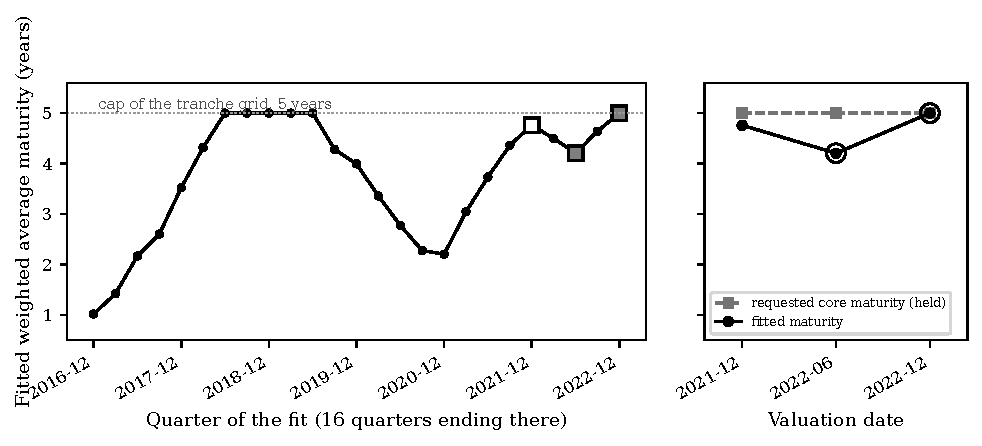
\includegraphics[width=0.92\textwidth]{history}
\caption{The weighted average maturity of the wholesale deposits fitted at each quarter from 2016-Q4 to 2022-Q4 on the last 16 quarters of the bank's deposit cost and of the Treasury tranche yields (left), with the three committed valuation dates marked and the two dates flagged by the proposed test ringed, and the series at those three dates beside the requested core maturity that the case holds fixed (right).}
\label{fig:history}
\end{figure}

Figure~\ref{fig:history} places the three dates in the full fitted series. The series has \realFits{} fits; its median absolute change between consecutive fits is \realMedianChange{} years and its largest is \realMaxChange{} years; \realZeroShare{} of the changes are zero, which happens where the solution sits at the 5-year cap of the tranche grid, and the weighted average maturity is at the cap at \realCapShare{} of the dates. The figure shows what Proposition~\ref{prop:degeneracy} states: a fitted series moves at nearly every date, so the red rows reflect the re-estimation and the breach, and not a decision. The two other behavioural tests of the engine, run on the committed inputs, read the same history differently. The stability test of the weights is red at 2021-Q4, with a largest sup-norm distance of \cOneFourStabStatA{} and a change of up to \cOneFourStabYearsA{} years in the weighted average maturity, amber at 2022-Q2 (\cOneFourStabStatB{}) and red at 2022-Q4 (\cOneFourStabStatC{}), so it flags the date at which the proposed test has nothing to say. The comparison of the economic value with and without the behavioural treatment is red at the three dates, with differences of \cOneFourWwStatA{} and \cOneFourWwStatC{} of Tier~1 at the first and the last, and none of them is a hidden breach, since the behavioural measure breaches the outlier test as well as the contractual one. None of the three tests reads the timing of an assumption against the timing of a breach except the proposed one, and on this case none can say whether the bank altered its assumptions, because the behaviour is synthetic.

\subsection{Constructed and enumerated histories}
\label{sec:res-constructed}

The engine agrees with the definition on all \constructedN{} constructed histories of Table~\ref{tab:constructed}, of which \constructedAgree{} gave the expected light: green for the parameter held through a breach, for the change with no breach, for the change before the breach and for a breach at the earlier date only; red for the change at the breach and for two changes at two breaches; not evaluated for a single date. Prediction H2 asks for more than examples, and the enumeration provides it: on every one of the \gridTotal{} histories of a binary grid of \gridLengths{} dates, each pattern of changes crossed with each pattern of flags (\gridSix{} histories of six dates), and on \randomN{} random histories with ties at a cap, the number of disagreements between the engine and Equation~\eqref{eq:count} is \gridBad{}. The light was red exactly when the count was positive in all of them.

\begin{table}[htbp]
\centering
\footnotesize
\caption{Constructed histories with a known answer, the parameter values and breach flags at three valuation dates, the light expected from the definition of the test and the light returned by the engine; the single-date history has one value and one flag.}
\label{tab:constructed}
\resizebox{\textwidth}{!}{%
\begin{tabular}{lllllr}
\toprule
History & Parameter & Breach flags & Expected & Engine & Flagged changes \\
\midrule
parameter held through a breach & $(4, 4, 4)$ & $(1, 1, 1)$ & green & green & 0 \\
change with no breach & $(4, 4.5, 5)$ & $(0, 0, 0)$ & green & green & 0 \\
change before the breach & $(4, 4.5, 4.5)$ & $(0, 0, 1)$ & green & green & 0 \\
change at the breach & $(4, 4, 4.5)$ & $(0, 0, 1)$ & red & red & 1 \\
breach at the earlier date only & $(4, 4.5, 4.5)$ & $(1, 0, 0)$ & green & green & 0 \\
two changes at two breaches & $(4, 4.5, 5)$ & $(0, 1, 1)$ & red & red & 2 \\
change at the first date (no previous date) & $(4, 4, 4)$ & $(1, 0, 0)$ & green & green & 0 \\
a single date & $(4)$ & $(1)$ & not evaluated & not evaluated & -- \\
\bottomrule
\end{tabular}}
\end{table}


Table~\ref{tab:last-digit} shows the convention the test inherits from its definition. A parameter held at 4 years with Gaussian noise of standard deviation $10^{-16}$ added at each date is still green, because the noise is smaller than the spacing of floating-point numbers at 4 and the sum rounds back; noise of \noiseFirstRed{} or more turns the light red at the two breach dates, and the held value recomputed as the sum of 0.1 and 0.2 differs from 0.3 in the last digit and is red too. A parameter that is recomputed at each date through a different order of operations, even if its mathematical value is constant, is flagged, so an implementation of the test on a stated parameter must hold it as the number that was decided and not as the result of a calculation.

\begin{table}[htbp]
\centering
\footnotesize
\caption{The effect of the last digit of a held parameter on the proposed test: a parameter held at 4 years through a 12-quarter history with two breach dates, to which Gaussian noise of the stated size is added at each date; the last row is the same value recomputed as 0.1 plus 0.2 and as 0.3, two floating-point numbers that differ.}
\label{tab:last-digit}
\begin{tabular}{lll}
\toprule
Noise on the held value (standard deviation) & Engine & Flagged changes \\
\midrule
0 & green & 0 \\
1e-16 & green & 0 \\
1e-13 & red & 2 \\
1e-09 & red & 2 \\
1e-06 & red & 2 \\
$0.1+0.2$ against $0.3$ & red & 2 \\
\bottomrule
\end{tabular}
\end{table}


\subsection{A stated parameter with planted changes}
\label{sec:res-stated}

Table~\ref{tab:main-results} gives the comparison in the base cell, with unrelated changes at 0.10 per quarter and a breach prevalence of 0.25, on \statedN{} histories per arm with a mean of \statedMeanM{} breach dates. The proposed test flags \statedAltEngine{} of the histories with a planted change at a breach date (lower end of the interval \statedAltLoEngine{}\,\%), as Proposition~\ref{prop:separation} requires, and \statedNullEngine{} (\statedNullLoEngine{} to \statedNullHiEngine{}\,\%) of the histories whose changes are unrelated to the breaches. The breach-agnostic count flags the same share of the alternative histories and \statedNullAny{} of the null ones, so the conjunction with the breach flag removes about half of the false flags at no cost in detection. The Fisher test flags \statedNullFisher{} of the null histories and \statedAltFisher{} of the alternative ones, the Mann--Whitney test \statedNullMw{} and \statedAltMw{}, and the Welch test \statedNullWelch{} and \statedAltWelch{}: they hold a size far below the nominal 5\,\% and detect a fraction of the planted changes. In the area under the ROC curve the ordering is not the same: the Fisher test (\statedAucFisher{}) and the Mann--Whitney test (\statedAucMw{}) rank the histories slightly better than the count of the proposed test (\statedAucEngine{}), which has only the values of its count to rank with, and the Welch test is lower (\statedAucWelch{}).

\begin{table*}[htbp]
\centering
\footnotesize
\caption{The proposed test and the comparators run on the same histories: on a stated parameter (4,000 histories per arm, changes unrelated to the breach at 0.10 per quarter, breach prevalence 0.25) and on a re-estimated parameter (2,000 banks, breach prevalence 0.25, a 2-year lengthening planted at breach dates); false-flag and detection rates with 95\% Wilson intervals, and the area under the ROC curve; the tolerance is calibrated at 5\% on 1,000 separate banks.}
\label{tab:main-results}
\resizebox{\textwidth}{!}{%
\begin{tabular}{lcccccc}
\toprule
\multicolumn{1}{l}{} & \multicolumn{3}{c}{Stated parameter} & \multicolumn{3}{c}{Re-estimated parameter} \\
\cmidrule(lr){2-4}\cmidrule(lr){5-7}
Detector & False flags (\%) & Detection (\%) & AUC & False flags (\%) & Detection of +2 years (\%) & AUC \\
\midrule
Proposed test & 34.8 (33.4, 36.3) & 100.0 (99.9, 100.0) & 0.908 & 82.2 (80.5, 83.9) & 100.0 (99.8, 100.0) & 0.579 \\
Any change & 68.8 (67.3, 70.2) & 100.0 (99.9, 100.0) & 0.863 & 92.5 (91.3, 93.6) & 100.0 (99.8, 100.0) & 0.536 \\
Fisher exact test & 0.1 (0.1, 0.3) & 13.2 (12.2, 14.3) & 0.922 & 2.1 (1.5, 2.8) & 4.1 (3.3, 5.1) & 0.596 \\
Mann--Whitney test & 2.6 (2.1, 3.1) & 48.0 (46.5, 49.6) & 0.914 & 7.2 (6.2, 8.5) & 31.4 (29.5, 33.5) & 0.796 \\
Welch test & 0.3 (0.2, 0.6) & 26.8 (25.5, 28.2) & 0.761 & 6.0 (5.1, 7.2) & 28.9 (27.0, 30.9) & 0.696 \\
Calibrated tolerance & -- & -- & -- & 3.9 (3.1, 4.8) & 18.0 (16.4, 19.7) & 0.937 \\
Calibrated tolerance, look-ahead & -- & -- & -- & 4.5 (3.6, 5.4) & 17.2 (15.6, 18.9) & 0.925 \\
Weight stability (engine) & -- & -- & -- & 49.8 (47.6, 52.0) & -- & -- \\
\bottomrule
\end{tabular}}
\end{table*}


The false-flag rate of the proposed test over the \statedCells{} cells of Table~\ref{tab:stated-grid} runs from \statedNullMin{} to \statedNullMax{}, at the lowest rate of unrelated changes with the lowest prevalence and at the highest with the highest, so prediction H5, a rate of at most 5\,\%, is refuted in every cell. Equation~\eqref{eq:false-flag}, evaluated with the number of breach dates of the very histories of each cell, lies inside the interval of the measured rate in \bernInside{} of the \bernCells{} cells (prediction H4); the cell outside, $\lambda=0.05$ at prevalence 0.5, has a closed form of \bernOutPred{} and a measured rate of \bernOutObs{}, a difference of \proofGap{} percentage points that is the largest of the grid, and under \bernExtraInside{} of three further seeds of 10,000 histories the closed form is inside the interval. The Fisher and Mann--Whitney tests never exceed \fisherNullMax{} and \mwNullMax{} false flags in any cell. The detection of the Fisher test depends on how many breach dates carry a planted change: with $\pi_m$ at 0.25, 0.5 and 1 it flags \piSweepAFisher{}, \piSweepBFisher{} and \piSweepCFisher{}, the Mann--Whitney test \piSweepAMw{}, \piSweepBMw{} and \piSweepCMw{}, and the Welch test \piSweepAWelch{}, \piSweepBWelch{} and \piSweepCWelch{}, whereas the proposed test flags every history in every cell (\statedAltMinLo{} at the lowest lower bound; prediction H3 holds).

\begin{table*}[htbp]
\centering
\footnotesize
\caption{The stated parameter over the grid of the rate of changes unrelated to the breach ($\lambda$ per quarter), the breach prevalence and the probability of a planted change at a breach date ($\pi_m$), 4,000 histories per arm in each row: the mean number $m$ of breach dates, the false-flag rate of the proposed test predicted by Proposition~\ref{prop:false-flag} and measured, and the detection rates of three detectors.}
\label{tab:stated-grid}
\resizebox{\textwidth}{!}{%
\begin{tabular}{rrrrrcrrr}
\toprule
\multicolumn{4}{l}{} & \multicolumn{2}{c}{Proposed test, false flags (\%)} & \multicolumn{3}{c}{Detection (\%)} \\
\cmidrule(lr){5-6}\cmidrule(lr){7-9}
$\lambda$ & Prevalence & $\pi_m$ & Mean $m$ & Closed form & Measured & Proposed & Fisher & Mann--Whitney \\
\midrule
0.05 & 0.10 & 0.50 & 3.87 & 17.2 & 17.0 (15.8, 18.1) & 100.0 & 13.5 & 57.4 \\
0.05 & 0.25 & 0.50 & 4.42 & 19.4 & 18.7 (17.5, 20.0) & 100.0 & 14.0 & 52.1 \\
0.05 & 0.50 & 0.50 & 5.80 & 25.0 & 27.4 (26.0, 28.8) & 100.0 & 16.3 & 39.5 \\
0.10 & 0.10 & 0.50 & 4.01 & 31.7 & 31.9 (30.4, 33.3) & 100.0 & 11.3 & 51.1 \\
0.10 & 0.25 & 0.50 & 4.37 & 34.3 & 34.8 (33.4, 36.3) & 100.0 & 13.2 & 48.0 \\
0.10 & 0.50 & 0.50 & 5.85 & 43.6 & 42.9 (41.4, 44.5) & 100.0 & 12.6 & 35.1 \\
0.20 & 0.10 & 0.50 & 3.92 & 51.3 & 52.0 (50.5, 53.5) & 100.0 & 8.8 & 43.9 \\
0.20 & 0.25 & 0.50 & 4.38 & 55.4 & 55.2 (53.7, 56.8) & 100.0 & 9.8 & 40.5 \\
0.20 & 0.50 & 0.50 & 5.73 & 66.5 & 66.3 (64.9, 67.8) & 100.0 & 10.2 & 31.8 \\
0.10 & 0.25 & 0.25 & 4.36 & 34.2 & 33.0 (31.6, 34.5) & 100.0 & 2.8 & 31.0 \\
0.10 & 0.25 & 1.00 & 4.48 & 34.8 & 34.1 (32.6, 35.6) & 100.0 & 60.2 & 89.1 \\
\bottomrule
\end{tabular}}
\end{table*}


\begin{figure}[htbp]
\centering
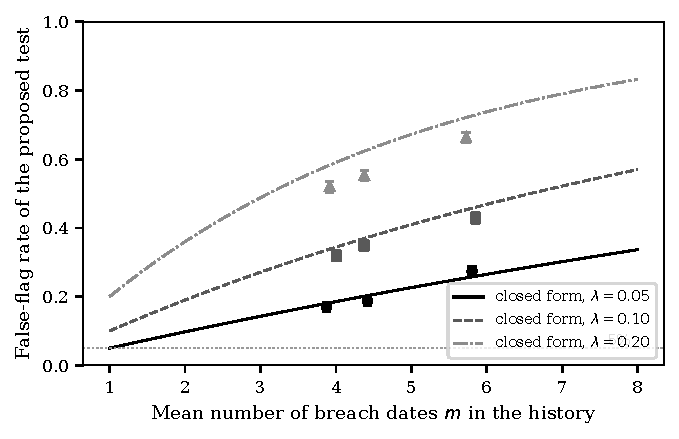
\includegraphics[width=0.62\textwidth]{false-flag}
\caption{The false-flag rate of the proposed test on a stated parameter against the mean number of breach dates in the history, for three rates of unrelated changes, with the closed form of Proposition~\ref{prop:false-flag} as lines and the nine cells of the simulation as markers with their 95\% Wilson intervals; the dotted line is a rate of 5\%.}
\label{fig:false-flag}
\end{figure}

Figure~\ref{fig:false-flag} shows the agreement of the closed form with the nine cells of the grid and the rise of the rate with the number of breach dates; the rate does not depend on the planted changes, which are absent from the null arm. Figure~\ref{fig:operating-points} plots the detection against the false-flag rate of the five detectors over the same cells. The proposed test and the breach-agnostic count sit on the line of full detection with false-flag rates between \statedNullMin{} and \statedNullAnyMax{}, and the three tests sit near the line of no false flags with detection between \opTestsMin{} and \opTestsMax{}; no detector reaches the corner of full detection at a low false-flag rate, because in a history of a dozen quarters a coincidence and a decision cannot be told apart by the dates alone. The figure does not show the tolerance rule, which is not defined on a stated parameter, where every change is a decision and the size of a change is a matter of governance and not of estimation.

\begin{figure}[htbp]
\centering
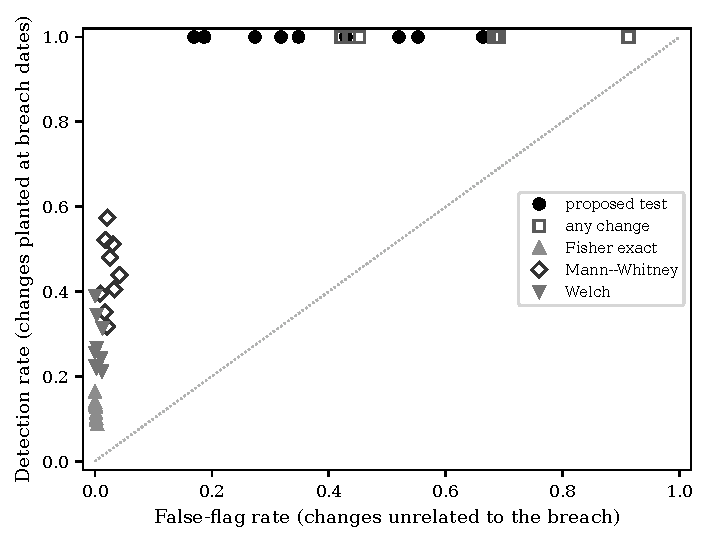
\includegraphics[width=0.66\textwidth]{operating-points}
\caption{Detection rate against false-flag rate of five detectors on a stated parameter, one marker for each of the nine cells of the grid of the rate of unrelated changes and the breach prevalence, with the proposed test at full detection and the three published tests near the line of no false flags.}
\label{fig:operating-points}
\end{figure}

\subsection{A re-estimated parameter}
\label{sec:res-fitted}

The simulated banks are block bootstraps of the real rows, and Table~\ref{tab:realism} compares their changes with those of the real fitted series. Their zero-change share (\simZero{}) and their share of dates at the cap (\simCap{}) are close to the real ones, and their largest change, \simMax{} years on average, is larger than the real \realMaxChange{} years; their median change, \simMedian{} years, is smaller than the real \realMedianChange{} years, which is above the 95th percentile of the simulated medians (\simMedianQNineFive{} years). The simulated changes are thus more often tiny and more often large than the real ones, which are steady, and Figure~\ref{fig:changes-ecdf} shows the distributions. The weight of this difference falls on the calibrated tolerance and is reported where it appears.

\begin{table}[htbp]
\centering
\footnotesize
\caption{The real fitted series of the bank (25 rolling fits from 2016-Q4 to 2022-Q4, and the last 12) against the simulated banks on the properties of the changes that the detectors read; the simulated banks are circular block bootstraps of the 40 real quarterly rows with blocks of 6 quarters.}
\label{tab:realism}
\resizebox{\textwidth}{!}{%
\begin{tabular}{lrrr}
\toprule
Property of the fitted weighted average maturity & Real, 25 fits & Real, last 12 fits & Simulated, mean of 2,000 banks \\
\midrule
Median absolute change (years) & 0.435 & 0.437 & 0.140 \\
Largest absolute change (years) & 0.919 & 0.843 & 1.116 \\
Share of dates with no change & 0.167 & 0.000 & 0.276 \\
Share of dates at the 5-year cap & 0.240 & 0.083 & 0.289 \\
Standard deviation of the level (years) & 1.198 & 0.943 & 0.714 \\
\bottomrule
\end{tabular}}
\end{table}


\begin{figure}[htbp]
\centering
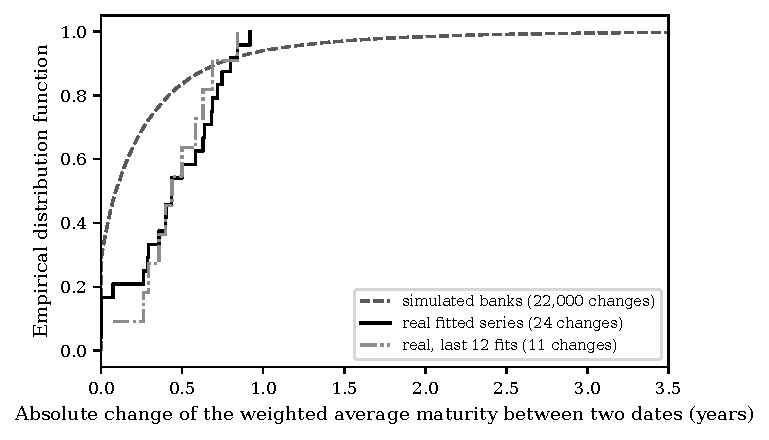
\includegraphics[width=0.62\textwidth]{changes-ecdf}
\caption{The empirical distribution of the absolute change of the fitted weighted average maturity between consecutive dates, for the 22,000 changes of the simulated test banks, the 24 changes of the real fitted series and the 11 changes of its last 12 fits.}
\label{fig:changes-ecdf}
\end{figure}

On the null banks, with a mean of \fitMeanM{} breach dates, the proposed test flags \fitNullEngine{} (\fitNullLoEngine{} to \fitNullHiEngine{}\,\%), and the \fitNullZero{} that it does not flag are those in which all the breach dates are ties, since \tieBanks{} of the banks have at least one tie at a breach date, \tieMean{} on average, because the weighted average maturity repeats at the cap. With a 2-year lengthening planted at breach dates it flags \fitAddCEngine{}, and the area under its ROC curve is \fitAucCEngine{} (\fitAucLoCEngine{} to \fitAucHiCEngine{}), the same at every size of the lengthening from 0.5 to 4 years, which is what Proposition~\ref{prop:degeneracy} predicts: the count is the number of breach dates minus the ties, and a planted change adds a change only where the fitted series was tied. Prediction H6, an area of at least 0.70, is refuted. The breach-agnostic count flags \fitNullAny{} of the null banks and has an area of \fitAucCAny{}. The stability test of the engine is red in \fitNullStab{} of the null banks, so a red result from it is no better evidence of an override. The published tests do better on ranking and worse on size: Table~\ref{tab:fitted-power} shows that the Mann--Whitney test flags \fitNullMw{} of the null banks, above its nominal 5\,\%, and \fitAddCMw{} of the banks with a 2-year lengthening, with an area of \fitAucCMw{}; the Welch test flags \fitNullWelch{} and \fitAddCWelch{}; the Fisher test flags \fitNullFisher{} and \fitAddCFisher{}.

\begin{table*}[htbp]
\centering
\footnotesize
\caption{Detection of a persistent lengthening of the fitted weighted average maturity planted at breach dates (breach prevalence 0.25): flag rate in percent and area under the ROC curve (separated by a slash) for each size of the lengthening, on 2,000 simulated banks and on 2,000 draws of breaches and overrides on the real fitted series of the bank; the tolerance is calibrated on the simulated banks.}
\label{tab:fitted-power}
\resizebox{\textwidth}{!}{%
\begin{tabular}{llrrrrr}
\toprule
Detector & Banks & False flags (\%) & +0.5 year & +1 year & +2 years & +4 years \\
\midrule
Proposed test & simulated & 82.2 & 100.0 / 0.58 & 100.0 / 0.58 & 100.0 / 0.58 & 100.0 / 0.58 \\
Proposed test & real series & 100.0 & 100.0 / 0.50 & 100.0 / 0.50 & 100.0 / 0.50 & 100.0 / 0.50 \\
Any change & simulated & 92.5 & 100.0 / 0.54 & 100.0 / 0.54 & 100.0 / 0.54 & 100.0 / 0.54 \\
Any change & real series & 100.0 & 100.0 / 0.50 & 100.0 / 0.50 & 100.0 / 0.50 & 100.0 / 0.50 \\
Fisher exact test & simulated & 2.1 & 4.1 / 0.60 & 4.1 / 0.60 & 4.1 / 0.60 & 4.2 / 0.60 \\
Fisher exact test & real series & 0.0 & 0.0 / 0.50 & 0.0 / 0.50 & 0.0 / 0.50 & 0.0 / 0.50 \\
Mann--Whitney test & simulated & 7.2 & 20.2 / 0.71 & 27.6 / 0.77 & 31.4 / 0.80 & 33.6 / 0.81 \\
Mann--Whitney test & real series & 4.4 & 8.4 / 0.58 & 20.5 / 0.76 & 28.0 / 0.82 & 28.0 / 0.82 \\
Welch test & simulated & 6.0 & 19.9 / 0.64 & 25.0 / 0.67 & 28.9 / 0.70 & 30.6 / 0.71 \\
Welch test & real series & 11.7 & 16.2 / 0.58 & 24.7 / 0.63 & 31.3 / 0.67 & 32.1 / 0.68 \\
Level-shift test (supremum t) & simulated & 5.9 & 6.8 / 0.65 & 6.2 / 0.71 & 8.4 / 0.76 & 13.1 / 0.79 \\
Level-shift test (supremum t) & real series & 0.0 & 0.0 / 0.71 & 0.4 / 0.67 & 8.1 / 0.64 & 13.8 / 0.57 \\
Level-shift test, break on a breach date & simulated & 6.2 & 14.1 / 0.66 & 18.1 / 0.73 & 25.1 / 0.78 & 32.9 / 0.83 \\
Level-shift test, break on a breach date & real series & 0.0 & 28.6 / 0.61 & 30.0 / 0.63 & 35.8 / 0.71 & 45.1 / 0.75 \\
Calibrated tolerance & simulated & 3.9 & 4.5 / 0.68 & 6.2 / 0.82 & 18.0 / 0.94 & 99.5 / 1.00 \\
Calibrated tolerance & real series & 0.0 & 0.0 / 0.80 & 0.0 / 0.88 & 42.9 / 1.00 & 100.0 / 1.00 \\
Calibrated tolerance, look-ahead & simulated & 4.5 & 5.1 / 0.65 & 6.6 / 0.79 & 17.2 / 0.93 & 99.4 / 0.99 \\
Calibrated tolerance, look-ahead & real series & 0.0 & 0.0 / 0.80 & 0.0 / 0.86 & 42.9 / 1.00 & 100.0 / 1.00 \\
\bottomrule
\end{tabular}}
\end{table*}


\begin{figure}[htbp]
\centering
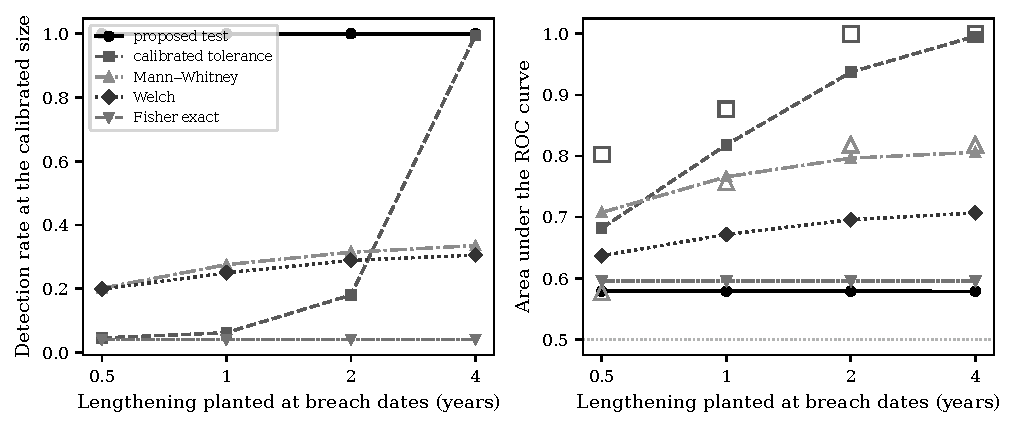
\includegraphics[width=0.95\textwidth]{fitted-power}
\caption{Detection rate at the calibrated size (left) and area under the ROC curve (right) against the size of a lengthening planted at breach dates, for the proposed test, the calibrated tolerance and three published tests on the simulated banks (lines), with the areas on the real fitted series for the tolerance and the Mann--Whitney test as open markers.}
\label{fig:fitted-power}
\end{figure}

Figure~\ref{fig:fitted-power} shows the same results as curves: the proposed test is flat at an area of \fitAucCEngine{} whatever the size of the lengthening, the published tests reach areas between \fitAucDFisher{} and \fitAucDMw{} at 4 years, and the tolerance rule passes them between 0.5 and 1 year and reaches \fitAucDTol{} at 4 years.

The tolerance rule restores the discrimination for overrides larger than the natural changes. Calibrated at 5\,\% on 1,000 separate banks at the breach prevalence of 0.25, its tolerance is \deltaB{} years and it flags \fitNullTol{} of the null banks (\fitNullLoTol{} to \fitNullHiTol{}\,\%), so the size holds (prediction H7). It flags \fitAddATol{}, \fitAddBTol{}, \fitAddCTol{} and \fitAddDTol{} of the banks with a lengthening of 0.5, 1, 2 and 4 years, and its areas are \fitAucATol{}, \fitAucBTol{}, \fitAucCTol{} and \fitAucDTol{}: at 1 year it flags only \fitAddBTol{}, at 2 years \fitAddCTol{} of the overrides, and at 4 years nearly all. The look-ahead variant is within one percentage point of it at every size. On the real fitted series, whose changes never exceed \realMaxChange{} years, the tolerance calibrated on the simulated banks is too large: it flags \realTolNull{} of the null draws, \realTolAddB{} of those with a 1-year lengthening, \realTolAddC{} of those with 2 years and \realTolAddD{} of those with 4 years, while its area is \realTolAucB{} at 1 year and \realTolAucC{} at 2 years. The threshold-free ranking is therefore excellent on the real series and the calibrated threshold is conservative, because the simulated population has larger changes than the real bank; the size is held and the power is lost. On the same draws the proposed test flags \realEngineNull{} of the null draws and has an area of \realEngineAuc{}, and the Mann--Whitney test flags \realMwNull{} of them with an area of \realMwAucC{} at 2 years.

The override that moves the weights toward the longest tranche (Table~\ref{tab:weight-override}) is the case that none of the detectors reads. In \invisShare{} of the histories the planted date finds the fitted weights already on the longest tranche, so that nothing changes; elsewhere the override lengthens the maturity by a fraction of the distance to the cap and shrinks every later change. The proposed test has an area of \wEngineAucLow{} at the smallest share and \wEngineAucHigh{} at the largest, below one half because the override creates ties; the stability test flags \wStabFlagHigh{} of the banks at the largest share with an area of \wStabAucHigh{}; the tolerance rule flags \wTolFlagHigh{} with an area of \wTolAucHigh{}, and the Mann--Whitney test has an area of \wMwAucHigh{}. This override is not detected by any method here, and it is the form that an override toward the cap of a standardised grid takes.

\begin{table*}[htbp]
\centering
\footnotesize
\caption{An override that moves the replicating-portfolio weights toward the longest tranche at breach dates (breach prevalence 0.25, 2,000 banks): the share of histories in which the override leaves the weights unchanged because they already sit on that tranche, and the flag rate and area under the ROC curve of the detectors that can read it.}
\label{tab:weight-override}
\resizebox{\textwidth}{!}{%
\begin{tabular}{rrrrrrrrr}
\toprule
Share $s$ & Invisible (\%) & Engine flags (\%) & Engine AUC & Stability flags (\%) & Stability AUC & Tolerance flags (\%) & Tolerance AUC & Mann--Whitney AUC \\
\midrule
0.05 & 22.1 & 83.4 & 0.506 & 47.6 & 0.483 & 3.2 & 0.498 & 0.519 \\
0.1 & 22.1 & 83.4 & 0.506 & 45.4 & 0.467 & 2.5 & 0.502 & 0.537 \\
0.2 & 22.1 & 83.0 & 0.498 & 40.6 & 0.442 & 2.4 & 0.521 & 0.576 \\
0.4 & 22.1 & 81.5 & 0.457 & 43.2 & 0.437 & 2.5 & 0.564 & 0.604 \\
\bottomrule
\end{tabular}}
\end{table*}


Table~\ref{tab:robustness} reports what happens when the breach prevalence of the bank is not that of the calibration. At the calibration prevalence of 0.25 the tolerance flags \fitNullBTol{} of the null banks; calibrated at the prevalence tested it flags \fitNullATol{} at 0.10 and \fitNullCTol{} at 0.50; calibrated at 0.25 and applied to the other prevalences it flags \fitMisATol{} and \fitMisCTol{} (upper end \fitMisCTolHi{} at 0.50), so the size is exceeded at the high prevalence and prediction H8, a rate of at most 5\,\% at every prevalence, is refuted by the point estimate while the interval includes 5\,\%. A tolerance rule is calibrated for a breach process and not for a bank. For the override one date before the planted breach, the tolerance flags \earlyTol{} of \earlyN{} banks and its look-ahead variant \earlyTolLa{}, a ratio of \earlyRatio{}, so prediction H9, a ratio of at least 1.5, is refuted; the proposed test and the breach-agnostic count flag \earlyEngine{} and \ablEarlyAny{}, which tells nothing about the override because they flag nearly all null banks.

\begin{table*}[htbp]
\centering
\footnotesize
\caption{False-flag rates on 2,000 held-out simulated banks at three breach prevalences: the tolerance rule calibrated on 1,000 banks at the prevalence tested and at 0.25 with 95\% Wilson intervals, and the published tests at their nominal 5\% size together with the red limit of the weight stability test.}
\label{tab:robustness}
\resizebox{\textwidth}{!}{%
\begin{tabular}{rrrccrrrr}
\toprule
\multicolumn{3}{l}{} & \multicolumn{2}{c}{Tolerance false flags (\%)} & \multicolumn{4}{c}{Other detectors, false flags (\%)} \\
\cmidrule(lr){4-5}\cmidrule(lr){6-9}
Prevalence & Mean $m$ & $\delta$ (years) & Calibrated here & Calibrated at 0.25 & Fisher & Mann--Whitney & Welch & Weight stability \\
\midrule
0.1 & 3.92 & 2.17 & 4.7 (3.9, 5.7) & 3.4 (2.7, 4.3) & 1.8 & 8.2 & 6.5 & 49.8 \\
0.25 & 4.41 & 2.47 & 3.9 (3.1, 4.8) & 3.9 (3.1, 4.8) & 2.1 & 7.2 & 6.0 & 49.8 \\
0.5 & 5.80 & 2.61 & 4.7 (3.9, 5.7) & 5.5 (4.6, 6.6) & 1.5 & 6.6 & 5.9 & 49.8 \\
\bottomrule
\end{tabular}}
\end{table*}


\subsection{Checks of the propositions}
\label{sec:res-theory}

Table~\ref{tab:theory-checks} compares the closed forms with simulation. The probability of Equation~\eqref{eq:hypergeometric} (Figure~\ref{fig:hypergeometric}) lies inside the interval of the simulated placement rate in \hyperInside{} of \hyperCells{} pairs $(k,m)$, and the one outside lies \hyperOutGap{} percentage points from its interval, as expected of \hyperCells{} 95\,\% intervals, which miss about one comparison in twenty. The detection probability of Equation~\eqref{eq:gaussian-power} differs from simulation by at most \gaussWorst{} over the \gaussPoints{} points of Figure~\ref{fig:gaussian-power}. The one-sided Fisher p-value equals the permutation p-value to within \fisherPermMax{} on \fisherPermN{} random histories (Proposition~\ref{prop:association}). The mean false-flag rate of the calibrated tolerance over \confCalibrations{} calibrations of \confNcal{} histories is \confMean{}, against \confTheory{} from Equation~\eqref{eq:conformal}; the realised rate of one calibration ranges from \confLo{} to \confHi{} (2.5th to 97.5th percentile), with a largest value of \confMax{}, and \confShareAbove{} of the calibrations exceed 5\,\%, as the bound on the average allows (Figure~\ref{fig:conformal-validity}).

\begin{table}[htbp]
\centering
\footnotesize
\caption{The closed forms of Propositions~\ref{prop:false-flag}, \ref{prop:gaussian} and \ref{prop:conformal} against simulation: the probability that a change falls on a breach date under uniform placement (100,000 placements), the power of the tolerance rule on Gaussian changes (200,000 histories) and the mean false-flag rate of the calibrated tolerance over 500 calibrations of 1,000 maxima of three Gaussian changes, with the 2.5 and 97.5 percentiles of the realised rate.}
\label{tab:theory-checks}
\begin{tabular}{lcc}
\toprule
Quantity & Closed form & Simulation (95\% interval) \\
\midrule
\relax Placement: $n=11$, $k=1$, $m=1$ & 0.0909 & 0.0925 (0.0907, 0.0943) \\
\relax Placement: $n=11$, $k=1$, $m=4$ & 0.3636 & 0.3644 (0.3614, 0.3674) \\
\relax Placement: $n=11$, $k=2$, $m=2$ & 0.3455 & 0.3460 (0.3430, 0.3489) \\
\relax Placement: $n=11$, $k=3$, $m=4$ & 0.7879 & 0.7873 (0.7847, 0.7898) \\
\relax Placement: $n=11$, $k=5$, $m=6$ & 0.9978 & 0.9975 (0.9971, 0.9978) \\
\relax Gaussian power: $m=1$, $\mu/\sigma=1$ & 0.1701 & 0.1693 \\
\relax Gaussian power: $m=1$, $\mu/\sigma=2$ & 0.5160 & 0.5151 \\
\relax Gaussian power: $m=1$, $\mu/\sigma=4$ & 0.9793 & 0.9794 \\
\relax Gaussian power: $m=3$, $\mu/\sigma=1$ & 0.1138 & 0.1138 \\
\relax Gaussian power: $m=3$, $\mu/\sigma=2$ & 0.3710 & 0.3690 \\
\relax Gaussian power: $m=3$, $\mu/\sigma=4$ & 0.9483 & 0.9477 \\
\relax Gaussian power: $m=6$, $\mu/\sigma=1$ & 0.0913 & 0.0919 \\
\relax Gaussian power: $m=6$, $\mu/\sigma=2$ & 0.2948 & 0.2969 \\
\relax Gaussian power: $m=6$, $\mu/\sigma=4$ & 0.9181 & 0.9189 \\
Calibrated tolerance: mean false-flag rate, 500 calibrations & 0.0500 & 0.0506 (0.0373, 0.0650) \\
\bottomrule
\end{tabular}
\end{table}


\begin{figure}[htbp]
\centering
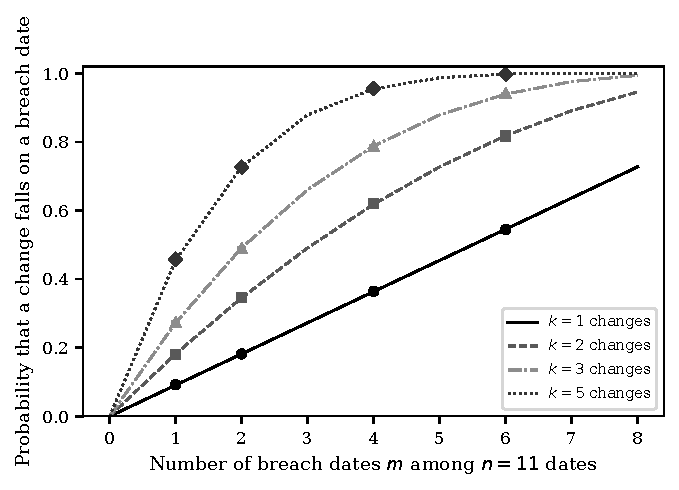
\includegraphics[width=0.62\textwidth]{hypergeometric}
\caption{The probability that at least one change falls on a breach date, from Equation~\eqref{eq:hypergeometric}, against the number of breach dates among 11 dates, for one, two, three and five changes (lines), with the simulated placements as markers and their 95\% Wilson intervals.}
\label{fig:hypergeometric}
\end{figure}

\begin{figure}[htbp]
\centering
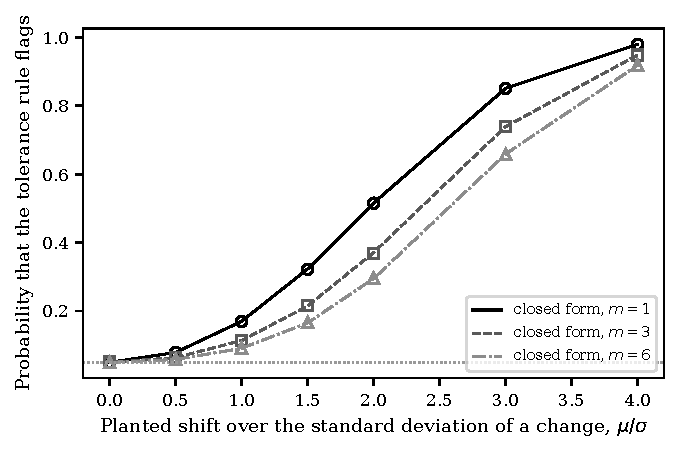
\includegraphics[width=0.62\textwidth]{gaussian-power}
\caption{The probability that the tolerance rule flags Gaussian changes against the planted shift in units of their standard deviation, for one, three and six breach dates, with the closed form of Equation~\eqref{eq:gaussian-power} as lines and the simulation as open markers; the dotted line is the size of 5\%.}
\label{fig:gaussian-power}
\end{figure}

\begin{figure}[htbp]
\centering
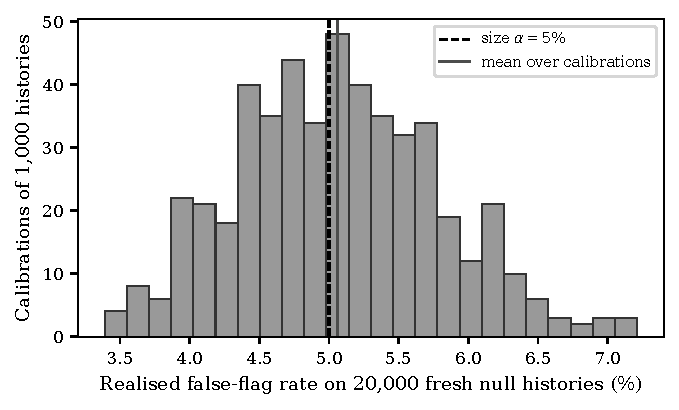
\includegraphics[width=0.62\textwidth]{conformal-validity}
\caption{The realised false-flag rate on \confNtest{} fresh null histories of each of \confCalibrations{} independent calibrations of the tolerance on \confNcal{} null histories each, with the size of 5\% and the mean over the calibrations marked.}
\label{fig:conformal-validity}
\end{figure}

\subsection{Outcome of the predictions}
\label{sec:res-hypotheses}

Table~\ref{tab:hypotheses} gives the nine predictions with their measured values: \hypothesesHeld{} held and \hypothesesRefuted{} were refuted. H1 to H4 and H7 held. H5, H6, H8 and H9 were refuted, and each refutation is a result about the limits of the test: its false-flag rate on a stated parameter is not at the conventional size, it does not discriminate on a re-estimated parameter, a calibrated tolerance does not transfer across breach prevalences without a loss of size, and reading one date ahead does not recover an anticipated override. The five that held are the specification of the test and the closed forms that follow from it: the reproduction of the committed rows and of the definition on every history enumerated, the detection of one on a stated parameter, the closed form of the false-flag rate, and the size of the calibrated tolerance together with its detection of large overrides. The four that failed are the predictions that a validator would make by treating the test as a statistical test of a re-estimated parameter, and each failure traces to a proposition: H5 to Proposition~\ref{prop:false-flag}(c), H6 to Proposition~\ref{prop:degeneracy}, H8 to the exchangeability that Proposition~\ref{prop:conformal} requires, and H9 to the single change that a persistent override produces. The outcomes are decided by code from the committed results, with the criteria of Table~\ref{tab:hypotheses}, so that a rerun that changed a rate across a criterion would change the outcome in the table.

\begin{table}[htbp]
\centering
\footnotesize
\caption{The nine predictions tested, with the criterion that decides each, the value measured by the experiments of this work and the outcome; the experiments are on the stored history of case C14, on constructed and enumerated histories and on 4,000 simulated histories per cell. A dagger marks a prediction formulated after a first run of the re-estimated experiment had been inspected (Section~\ref{sec:design-hypotheses}).}
\label{tab:hypotheses}
\begin{tabular}{@{}l p{4.6cm} p{3.2cm} p{3.1cm} l@{}}
\toprule
ID & Prediction & Criterion & Measured & Outcome \\
\midrule
H1 & The test is not evaluated at 2021-Q4, red at 2022-Q2 with one change and red at 2022-Q4 with two; the held core share and core maturity are not flagged & all three stored rows and the two held parameters reproduced by the engine on the stored series & 3 of 3 rows; 2 of 2 held parameters & held \\
H2 & Green for a parameter held through a breach, for a change with no breach and for a change before the breach; red for a change at the breach; the stored series with its breach flags set to false is green & all constructed histories, every history of a binary grid, 20,000 random histories and the control agree with the closed-form count & 8 of 8 histories; 0 disagreements in 22,728 & held \\
H3 & On a stated parameter the test flags every history in which an assumption was changed at a breach date & lower end of the 95\% interval of the detection at least 99\% in every cell & lowest lower bound 99.9\% over 11 cells & held \\
H4 & The false-flag rate on a stated parameter with changes unrelated to breaches equals $E[1-(1-\lambda)^m]$ (Proposition~\ref{prop:false-flag}) & the closed form inside the 95\% interval of the measured rate in at least 10 of 11 cells (an interval misses one cell in twenty), a cell outside re-run under three further seeds & 10 of 11 cells; the one outside inside the interval under 3 of 3 further seeds & held \\
H5 & The false-flag rate of the test on a stated parameter with unrelated changes is at most 5\% & the point estimate at most 5\% in every cell & 17.0 to 66.3\% & refuted \\
H6$^\dagger$ & On a re-estimated parameter the test separates a 2-year override at breach dates from none & area under the ROC curve at least 0.70 & 0.579 (0.561, 0.595) & refuted \\
H7$^\dagger$ & The tolerance rule calibrated at 5\% holds its size on held-out banks and flags a 4-year override & false-flag rate at most 5\% and detection of at least 90\% & 3.9\% false flags; 99.5\% detection & held \\
H8$^\dagger$ & The tolerance calibrated at breach prevalence 0.25 keeps its size at prevalences 0.10 and 0.50 & point estimate of the false-flag rate at most 5\% at every prevalence & 3.4 to 5.5\% (at 0.50, 95\% interval 4.6 to 6.6\%) & refuted \\
H9$^\dagger$ & A one-date look-ahead recovers a 4-year override made at the date before a breach begins & detection at least 1.5 times that of the same-date rule & 91.0\% against 3.7\% (ratio 24.9) & held \\
\bottomrule
\end{tabular}
\end{table}


\section{Ablation}
\label{sec:ablation}

Table~\ref{tab:ablation} removes or replaces one component of the proposed test at a time and reads the effect on the stated population and on the re-estimated one, in the base cells of Table~\ref{tab:main-results}, with a 2-year lengthening for the re-estimated parameter and a 2-year lengthening made one date early in the last column. The components are the conjunction with the breach flag, the exact inequality as the definition of a change, the same-date rule, and the counting statistic.

\begin{table*}[htbp]
\centering
\footnotesize
\caption{Ablation of the proposed test: each row removes or replaces one component (the conjunction with the breach flag, the exact inequality as the definition of a change, the same-date rule, the counting statistic) and reports the false-flag rate, the detection rate and the area under the ROC curve on the stated parameter and, for a 2-year lengthening, on the fitted parameter, and the detection of a 4-year lengthening made at the date before a breach begins.}
\label{tab:ablation}
\resizebox{\textwidth}{!}{%
\begin{tabular}{lccccccc}
\toprule
\multicolumn{1}{l}{} & \multicolumn{3}{c}{Stated parameter} & \multicolumn{3}{c}{Re-estimated parameter} & \multicolumn{1}{c}{Detection} \\
\cmidrule(lr){2-4}\cmidrule(lr){5-7}\cmidrule(lr){8-8}
Variant of the method & False flags (\%) & Detection (\%) & AUC & False flags (\%) & Detection (\%) & AUC & Override before the breach (\%) \\
\midrule
Proposed test as implemented: exact change, breach conjunction, same date & 34.8 & 100.0 & 0.908 & 82.2 & 100.0 & 0.579 & 81.9 \\
Without the breach conjunction (any change) & 68.8 & 100.0 & 0.863 & 92.5 & 100.0 & 0.536 & 100.0 \\
Exact change replaced by a calibrated tolerance & -- & -- & -- & 3.9 & 18.0 & 0.937 & 3.6 \\
Calibrated tolerance with a one-date look-ahead & -- & -- & -- & 4.5 & 17.2 & 0.925 & 98.6 \\
Counting replaced by an association test (Fisher) & 0.1 & 13.2 & 0.922 & 2.1 & 4.1 & 0.596 & 0.8 \\
Counting replaced by a rank test of the size of the changes (Mann--Whitney) & 2.6 & 48.0 & 0.914 & 7.2 & 31.4 & 0.796 & 1.5 \\
Counting replaced by a test for a shift in the level, whatever the breach flags & 4.0 & 5.8 & 0.796 & 5.9 & 8.4 & 0.756 & 42.0 \\
Counting replaced by a test for a shift in the level that falls on a breach date & 4.1 & 6.8 & 0.824 & 6.2 & 25.1 & 0.782 & 0.9 \\
\bottomrule
\end{tabular}}
\end{table*}


The conjunction with the breach flag is what separates the test from a monitor of parameter stability. Without it, the rule flags any history in which the parameter changed, and on the stated population the false-flag rate rises from \statedNullEngine{} to \statedNullAny{} at an unchanged detection of \statedAltAny{}; on the re-estimated population it rises from \fitNullEngine{} to \fitNullAny{} and the area under the ROC curve falls from \fitAucCEngine{} to \fitAucCAny{}. The component contributes specificity at no cost in detection, which is the reason to read the flags, and it contributes little on a re-estimated parameter, where almost every history has a change.

The exact inequality is the component with the two faces. On a stated parameter it is what gives the detection of one, since any change at all, however small, is a decision. On a re-estimated parameter it is what removes the discrimination: with the exact inequality the rule flags \fitNullEngine{} of the null banks and \fitAddCEngine{} of those with a 2-year lengthening, and replacing it by the tolerance calibrated at 5\,\% gives \fitNullTol{} and \fitAddCTol{} with an area of \fitAucCTol{}. The tolerance buys a stated size and a usable ranking at the price of the detection of small overrides, and it is the only variant that reads the size of a change at all. The same-date rule, replaced by the one-date look-ahead, does not help against an override made one date before the breach (\earlyTolLa{} against \earlyTol{} for the tolerance), because a persistent override produces one change at the date it is made and the look-ahead only widens the set of dates that can carry it by one; the cost is a small rise of the false-flag rate (\fitNullTolLa{} against \fitNullTol{}).

Replacing the count by an association test, the Fisher test, or by a rank test of the size of the changes, the Mann--Whitney test, trades detection for specificity. On the stated population they flag \statedNullFisher{} and \statedNullMw{} of the null histories and \statedAltFisher{} and \statedAltMw{} of the alternative ones, with areas of \statedAucFisher{} and \statedAucMw{}, against \statedAucEngine{} for the count: the tests rank slightly better and decide very differently, because the count has a decision at one coincidence and the tests need evidence that grows with the number of breach dates. On the re-estimated population the Mann--Whitney test has the largest area of the three published tests, \fitAucCMw{}, with a false-flag rate of \fitNullMw{} that exceeds its nominal level.

The ablation supports three readings. The conjunction with the flag and the exactness are both needed for the property that matters on a stated parameter, a flag that is certain for a change at a breach date and absent otherwise. The exactness has to be given up, for a tolerance read from a null, on a re-estimated parameter. And no component recovers an override that the data hide, as the override toward the longest tranche of Table~\ref{tab:weight-override} shows.

\section{Discussion}
\label{sec:discussion}

\subsection{Why the results are what they are}
\label{sec:disc-why}

The results follow from one property of the test, that it reads a change as an event with no size, and from the kind of parameter it reads. A stated parameter changes only when someone decides, so the indicator of a change is a record of decisions, and a coincidence of a decision with a breach is the event the test is built to see. The detection of one, in every cell, is the arithmetic of Proposition~\ref{prop:separation} and not an empirical finding about banks, and its value is that it holds without a model of the parameter. The false flags are the other side of the same arithmetic: a decision that happens to fall on a breach date is indistinguishable from one made because of it, so the false-flag rate is set by how busy the governance calendar is ($\lambda$) and how long the breach lasts ($m$), and it is not a property of the test that can be tuned. A re-estimated parameter changes at every date because the window moves, so the indicator of a change records the arithmetic of the estimator and the coincidence with a breach is the coincidence with a quarter-end. The degeneracy is then complete up to the ties at the cap, which is why the area under the ROC curve of the count against a planted override is \fitAucCEngine{} and does not move with the size of the override.

The tolerance rule works for the reason a tolerance always does: it replaces the question whether the parameter changed by the question whether it changed by more than the estimator changes it. Its power is the power of the maximum of the changes at the breach dates against a null whose maximum is read from a population, and Proposition~\ref{prop:gaussian} shows that this power rises slowly with the size of the override in units of the natural change and falls with the number of breach dates, as the experiments find: at the tolerance of \deltaB{} years the detection is \fitAddCTol{} at 2 years and \fitAddDTol{} at 4. The conformal calibration holds the size on average, and its size at a different breach prevalence depends on the exchangeability that the proposition names; the measured departure, \fitMisCTol{} against 5\,\% at a prevalence of 0.50, is inside the spread of a single calibration. On the real series the tolerance is conservative because the simulated population has changes larger than the real ones; the ranking is perfect at 2 years and the calibrated threshold is too high. Both facts have the same cause and the same remedy, a null population closer to the bank than a block bootstrap of its own rows.

\subsection{What a red light means and how to use the test}
\label{sec:disc-use}

On a stated parameter a red light means that an assumption was changed at a date at which a limit was breached. It does not mean that the change was made because of the breach, and Equation~\eqref{eq:false-flag} says how often it was not: at the rate of unrelated changes of the base cell and a mean of \statedMeanM{} breach dates, \statedNullEngine{} of the histories with no planted change are red. The right use is the one the engine's documentation gives, a prompt for a review of the minutes and the model file at the flagged date, with the false-flag rate read from the closed form for the bank's own governance calendar. A green light on a stated parameter is stronger evidence than a red one: no decision of any size was made at a breach date, which is a fact about the file and not about a distribution.

On a re-estimated parameter the exact test should not be used as a finding. The stored rows of case C14 are red because the weighted average maturity is fitted afresh at each date and the limit is breached at each, and the product's statement that those rows show the test operating on the parameter, and not that the bank altered anything, is the correct reading and follows from Proposition~\ref{prop:degeneracy}. Two uses remain. The first is to apply the test to the parameter that the bank states, the core maturity or the overlay that it adds to the fit, and not to the fit; for a bank that holds an override on top of a fitted value, the history of the override is a stated parameter. The second is the tolerance rule on the fit, calibrated on a null population of banks with the same estimator, length and breach process, and read as a ranking of how large the largest change at a breach date is relative to what the estimator produces; its value is the area under the ROC curve, and a threshold is a choice of a false-flag rate. Neither of these is implemented in the engine, which has the exact test only, and the second needs a population that a single validator may not have. The weight stability test of the engine is the existing check of the fit and it is red in about half of the null banks, so it too says more about the estimator than about the bank.

\subsection{Negative results and their implications}
\label{sec:disc-negative}

Three predictions were refuted and one family of overrides was detected only weakly by every method on the simulated banks and moderately by a test of the level on the real series. The refutation of H5 means that the test cannot be presented as a hypothesis test with a conventional size; it is a screen whose false-flag rate depends on the calendar. The refutation of H6 means that its output on a fitted parameter says little about an override: its area of \fitAucCEngine{} comes from the ties of the estimate at its cap, and it is \realEngineAuc{} on the real fitted series. H8 fails on its point estimate, \fitMisCTol{} (\fitMisCTolLo{} to \fitMisCTolHi{}\,\%) at a prevalence of 0.50 for a tolerance calibrated at 0.25, which is inside the spread of a single calibration; the data show the direction and not a loss of size beyond what the sampling of a calibration produces: a bank whose limit is breached more often needs a larger tolerance (\deltaA{}, \deltaB{} and \deltaC{} years at the three prevalences), since the maximum is taken over more dates. The result for H9 means that the dating convention, by which a change counts only at the date whose window contains the breach, is what keeps an anticipated override from being seen: a persistent override made at the date before a breach begins produces one change, at a date that is not a breach date, which the same-date rule cannot count and the look-ahead variant can, provided the change is larger than what the estimator produces, since the variant is a tolerance rule. The override toward the longest tranche is invisible in about a fifth of the histories because the fitted weights already sit there, and its effect on the others is a small lengthening and a damping of later changes; on the simulated banks no detector that reads the series exceeds an area of \wTopAuc{}, while on the real series, whose changes are steadier, a test of a shift in the level reaches \wRealTopAuc{}. A validator who wants to see such an override can therefore read the level of the series with a break test, which the tests of the changes do not do; whether reading the weights themselves, against the weights that the unconstrained fit would give, would see more of it was not tested here (the stability test of the engine, which reads them, reaches \realWAucStab{} on the real series). These results are not defects of the implementation. They are the properties of a coincidence rule, and the measured rates give a validator the numbers needed to decide how much weight a red or a green light deserves on a given parameter.

\section{Limitations}
\label{sec:limitations}

\subsection{Internal validity}
\label{sec:lim-internal}

The detection and false-flag rates are properties of the generators of histories, and the generators encode the assumptions of the experiments. The planted change is a persistent lengthening added at each breach date with probability $\pi_m$ and at least once, of 0.5 to 2 years on a stated parameter and of 0.5 to 4 years on a fitted one, and the unrelated changes of a stated parameter are independent across dates with a common probability. A bank whose unrelated changes cluster at the dates of the governance calendar, or whose override is made in several small steps, would give other rates; Proposition~\ref{prop:false-flag} covers the first case only with a $\lambda_t$ that varies, and the experiments do not. The breach chain has one persistence, and the closed forms and the measured rates depend on it through the number of breach dates. The comparators were run at their conventional settings: the Mann--Whitney test uses its asymptotic form, which is approximate for histories with many ties and for a dozen dates, and its measured size of \fitNullAMw{} to \fitNullCMw{} on the re-estimated population is above the nominal 5\,\%, whereas the Welch and Fisher tests are conservative or close to nominal. The change-point methods of Section~\ref{sec:related-work} are not included as separate detectors, because they have no input for the breach flags; the breach-agnostic count stands for them, and a method that estimated a break at an unknown date and then asked whether it fell on a breach would be a different test. The areas under the ROC curve are estimated on one set of 2,000 banks with a bootstrap interval, and the rates on five blocks whose standard deviations are in the committed results.

\subsection{External validity}
\label{sec:lim-external}

The committed history is one bank at three dates, and its behaviour is synthetic: no result here says what the bank did, and none says that a bank that follows the supervisory finding would be flagged. The simulated banks are block bootstraps of the 40 real quarterly rows of one bank in one regime, a decade of low and then rapidly rising rates, with blocks of six quarters, and the comparison with the real fitted series shows that they have more tiny and more large changes than the real series, which sits at the 95th percentile of the simulated median change. The calibrated tolerance inherits that mismatch: it holds its size on the simulated banks and is conservative on the real series. The block length was fixed before any detection experiment and was not tuned to the detection results; another length would move the tolerance. The histories are twelve quarters long (twenty-five on the real series, of which twelve are used), the number of breach dates is of the order of four, and a validator with a longer history or a different number of breach dates would face other rates; the closed forms show how, and the calibration has to be redone. The replicating portfolio of seven tranches with a 16-quarter window is the estimator of the product, and a bank with a different estimator, a deposit beta fitted on a different window, or a stochastic model of the deposit, would have a different distribution of changes and, perhaps, no ties at all.

\subsection{Construct validity and scope}
\label{sec:lim-construct}

A coincidence is not intent. The test measures the coincidence of a change with a flag, and the flag is a model output, the outlier ratio of a standardised shock, and not a limit that a committee set and recorded; a bank whose internal limit framework differs from the standard would give other flags. The dating convention, in which the flag of a date concerns the window ending there, is a choice, and an assumption changed in anticipation of a breach is by definition not a coincidence. The test sees only the parameters that are supplied to it: an assumption that is changed together with another, or replaced by a different parametrisation, is seen only if the series supplied reflects it. The internal gate that turns a count into a red light is the product's own and is not a regulatory limit. The tolerance family and its calibration are evaluated here and are not in the engine, so no claim of this paper concerns a released implementation of them. Finally, the absence claim of the introduction, that no published test of this kind was found, is bounded by the documents read; it is not a statement that none exists.

\section{Reproducibility}
\label{sec:reproducibility}

The code, the committed results and the data pipeline are in the repository \url{https://github.com/fsantibanezleal/CAOS_Contraste}, and the engine is the package \texttt{riskvalidation} 1.1.0 on the Python package index \citep{riskvalidation2026}. The experiments are scripts under \path{manuscripts/behavioural-assumption-test-at-a-limit-breach/experiments/}, run from the repository root with the Python environment of the product (\texttt{riskvalidation} 1.1.0 with the market, machine-learning and stress extras, and the requirements of the pipeline): \texttt{run\_reproduction.py} writes the committed-history and enumeration results, \texttt{run\_stated.py} the stated population, \texttt{run\_fitted.py} the re-estimated population and the real-series draws, and \texttt{run\_theory.py} the checks of the propositions. Each writes a JSON document next to it, \texttt{results\_reproduction.json}, \texttt{results\_stated.json}, \texttt{results\_fitted.json} and \texttt{results\_theory.json}, which are committed; the scripts draw every random number from the seeds in those documents and a rerun reproduces them. The unit tests of the shared core, \texttt{test\_core.py}, check the engine against the closed-form count, the statistics, the generators and the decision rules. The tables and the numbers of the text are written by \texttt{make\_tables.py} into \texttt{tables/}, including \texttt{tables/numbers.tex}, which defines one macro for each number quoted in the prose and records its source; the figures are written by \texttt{make\_figures.py} into \texttt{figures/} as vector files.

The raw inputs of case C14, the call-report file of the FDIC and the Treasury yield files, are read from the data root of the device (the environment variable \texttt{CONTRASTE\_DATA}) and are identified by the digests of the committed documents; the committed documents under \texttt{data/derived/C14/} are the other input. Every script runs in under 30 minutes on a workstation with 32 cores, the re-estimated population being the longest because it fits the replicating portfolio on every window of every bank, and the cache of the fitted weights, which is not committed, is written to the temporary root of the device and rebuilt when absent. The document is built with \texttt{pdflatex} and \texttt{bibtex} from the manuscript folder.

\section{Conclusions}
\label{sec:conclusions}

A test that counts the dates at which a behavioural parameter changed while a limit was breached turns a supervisory finding into a procedure with a known behaviour. On a parameter that a bank states and holds, it flags every change made at a breach date (\statedAltEngine{} of \statedN{} histories in the base cell, \statedAltMinLo{} at the lowest lower bound over \statedCells{} cells), it is silent when no change is made at a breach date, and it reproduces the stored rows of case C14 and agrees with its definition on \gridTotal{} enumerated and \randomN{} random histories. Its false-flag rate on unrelated changes is not a size to be chosen: it is $1-(1-\lambda)^m$ in expectation, from \statedNullMin{} to \statedNullMax{} over the cells measured, and the Fisher, Mann--Whitney and Welch tests, which hold a size below the nominal, detect only \opTestsMin{} to \opTestsMax{} of the planted changes at half of the breach dates at those lengths of history.

On a parameter that is re-estimated at each date, the exact test is red whenever a breach exists, up to the ties where the estimate sits at its cap: it flags \fitNullEngine{} of the null banks and its area against a planted override is \fitAucCEngine{}. The red rows of the stored case are therefore a statement about the estimator, as the product says, and they follow from Proposition~\ref{prop:degeneracy}. A tolerance on the size of a change, calibrated on a null population by a rank rule that holds its size on average in finite samples, restores the discrimination for overrides larger than the natural changes: \fitNullTol{} false flags and \fitAddDTol{} detection of a 4-year lengthening, with an area of \fitAucDTol{}. Calibrated at a breach prevalence of 0.25 and applied at 0.50 it flags \fitMisCTol{} of the null banks (\fitMisCTolLo{} to \fitMisCTolHi{}\,\%), a departure from 5\,\% that is inside the spread of a single calibration, so the size is held to within what a calibration can show; it is conservative on the real series; and an override toward the longest tranche is detected weakly on the simulated banks (no area above \wTopAuc{}, that of the break rule) and moderately on the real series (\wRealTopAuc{} for the level-shift test). The published test of a break at an unknown date, with the requirement that the break fall on a breach date, flags \fitAddCShiftB{} and \fitAddDShiftB{} of the 2- and 4-year lengthenings at \fitNullShiftB{} false flags, above 5\,\%, and \fitMisCShiftB{} (\fitMisCShiftBLo{} to \fitMisCShiftBHi{}\,\%) when it is calibrated at 0.25 and applied at 0.50, outside the spread of a calibration: the tolerance, at \fitNullTol{} false flags, ranks them better at both sizes and flags more of the 4-year ones. Three of the nine predictions failed: the conventional size on a stated parameter (H5), a ranking of a re-estimated parameter at the area predicted (H6) and, by its point estimate, the transfer of a tolerance across breach prevalences (H8).

The next steps follow from these limits. The first is to apply the exact test to the parameters that a bank states, including the overlay it adds to a fitted value, and to report its false-flag rate for the bank's own calendar from Equation~\eqref{eq:false-flag}. The second is to implement the tolerance rule with a calibration on a null population built from the bank's own estimator and breach process, and to test it on histories with a known override. The third is to extend the experiments to a longer panel of banks with their recorded limit frameworks, so that the rates are measured where the behaviour is real.


\bibliographystyle{plainnat}
\bibliography{references}

\end{document}
